\documentclass{article}

% Set up data, if you need to add a package, go here
%Adapted from Adapted from UWA Engineering Final Year Project.


\usepackage[utf8]{inputenc}
\usepackage[x11names,dvipsnames,svgnames,table]{xcolor}

% general incantations
\usepackage[export]{adjustbox}
\usepackage{afterpage}

\usepackage{graphicx}
\usepackage{placeins}
\usepackage{pdfpages}
\usepackage{algorithm2e}
\usepackage{array}
\usepackage{booktabs}
\usepackage[most]{tcolorbox}
\usepackage{calligra}
\usepackage{caption}
\usepackage{datetime}
\usepackage{dblfnote}
\usepackage{dirtytalk}
\usepackage{dsfont}
\usepackage{etex}
\usepackage{fancyhdr}
\usepackage{fix-cm}
\usepackage[T1]{fontenc}
\usepackage{textcomp,gensymb} %for \degree C symbol
\usepackage{graphicx}
\usepackage{lipsum}
\usepackage{listings}
\usepackage{transparent}
\usepackage[everyline=true,framemethod=tikz]{mdframed}
\usepackage{mparhack}
\usepackage{multicol}
\usepackage{multirow}
\usepackage{parskip}
\usepackage{lscape}
\usepackage{pdflscape}
\usepackage{pdfpages}
\usepackage{placeins}
\usepackage[document]{ragged2e}
\usepackage{rotating}
\usepackage{setspace}
\usepackage{subcaption}
\usepackage{threeparttable}
\usepackage[normalem]{ulem}
\usepackage{verbatim}
\usepackage{soul} %highlighting, strike through etc.
%Automated appendices
\usepackage[titletoc,title,header]{appendix} %advanced functionality

%language settings
\usepackage[utf8]{inputenc}
\usepackage[australian]{babel}
\usepackage{csquotes}

%page setup
%this where we adjust the binding offset, if relevant
\usepackage[a4paper]{geometry}
\usepackage{lastpage} % for page 1 of n footers

%cross referencing
\usepackage[hidelinks]{hyperref}
\usepackage{cleveref}

%maths stuff
\usepackage{amsmath}
\usepackage{mathtools}

\setcounter{secnumdepth}{5}

%lists
\usepackage{enumitem}


%working collaboratively
\usepackage[backgroundcolor=yellow]{todonotes}

% bibliography file using harvard
\usepackage[style=authoryear-ibid,backend=biber]{biblatex}
% \renewcommand*{\bibfont}{\small}
\renewcommand*{\bibfont}{\scriptsize}
\bibliography{bibliography.bib} % with extension



%glossary for acronyms
\usepackage[acronym,nonumberlist,toc,section=subsection,numberedsection=nolabel]{glossaries} 
\makeglossaries

%line spacing
\linespread{1.25}

\hypersetup{
    colorlinks=true,
    linkcolor=blue,
    filecolor=blue,
    citecolor=black,
    urlcolor=blue
    }


\begin{document}


\thispagestyle{empty}
\setlength\headheight{0pt} 
\begin{center}

\begin{center}

\includegraphics[width=0.65\linewidth]{images/TUD_Logo.png}            
\end{center}	

        \vspace{0.25cm}
        {\scshape\LARGE TU Dublin, Tallaght Campus \par}
        \vspace{0.25cm}
        {\scshape\Large MSc DevOps\par}
        {\scshape\Large Research Project }
        \vspace{0.5cm}

        {\Large\bfseries Knatve Vs Azure Function\par}
        
        \vspace{0.5cm}
        {\Large\itshape Ainul Habib\par}
        {\scshape\small X00159358 \par}
        Department of Computing
        \vspace{0.25cm}

\vspace{1cm}
Supervised by\par
GARY CLYNCH \\
Department of Computing\par
\large
\today

\end{center}

\clearpage
\restoregeometry
\justify

\section*{Declaration}
\begin{flushleft}
I hereby certify that the material, which I now submit for assessment on the programmes of study leading to the award of Master of Science, is entirely my own work and has not been taken from the work of others except to the extent that such work has been cited and acknowledged within the text of my own work. No portion of the work contained in this thesis has been submitted in support of an application for another degree or qualification to this or any other institution.
\end{flushleft}
\vspace{2cm}
\begin{flushright}
-----------------------------------\\
Ainul Habib\\
\today
\end{flushright}
\pagebreak

\section*{Acknowledgements}
 
 I would like to express my sincere gratitude to my supervisor, Gary Clynch, for his invaluable guidance and support throughout the research process. His expertise and insights have been instrumental in shaping this thesis.

I would also like to thank other faculties of the University and Programme, for their encouragement and support. Their feedback and suggestions have been invaluable in refining my research.

I am grateful to my family for their unwavering support and encouragement throughout this journey. Their love and encouragement have been a constant source of inspiration.

Finally, I would like to thank the participants of this study for their time and willingness to share their experiences. Without their participation, this research would not have been possible.
\pagebreak

%List of figures and tables, automatic from thesis.
\listoffigures
\pagebreak
 
% \listoftables
% \pagebreak

\pagebreak
\tableofcontents
\pagebreak


\section{Abstract}
\begin{flushleft}
Serverless computing technology provided the technological infrastructure that made the evolution of cloud computing from \gls{VM}(s) and containerized services (\gls{CAAS}) to just a “Function as a Service” (\gls{FAAS}). This paradigm shift brought simplification of Microservices design, and abstraction for infrastructure and server overheads.

Apart from all the goodies of Serverless, it provides a very real possibility for customers to get in a “locked-in” with a particular provider. 

\begin{quote}
    \textit{While the existing cloud solutions for public and private companies are vendor-locked-in by design, their existence is subject to the limited possibility of interoperating with other cloud systems.}\\
    \cite{Opara-Martins-2014} 
\end{quote}

The Serverless market needs a standardization, and unification by way of API offering and runtime contracts, to free developers from the fear of vendor lock-in. 

Knative is an Open-Source, Cloud-Native, Serverless offering, that extends Kubernetes (, a widly accepted \gls{PAAS},) with Serverless features. 

Azure Functions is a cloud-based service that provides event-driven and compute-on-demand capabilities for various Azure or third-party services. 

We evaluate both platforms based on several criteria, such as performance, cost, ease of use, portability, and ecosystem. We also present a case study of a real-world application that uses both platforms and discuss the challenges and benefits of each approach. 

Our results show that Azure Functions offers a more mature and integrated solution for Serverless computing, while Knative provides more flexibility and control for developers who want to leverage the power of Kubernetes.
\end{flushleft}

\pagebreak

\section{Introduction}
\begin{flushleft} 
In recent years, the landscape of cloud-native application development has witnessed a significant transformation, driven by the need for enhanced scalability, rapid deployment, and cost efficiency. As organizations strive to deliver seamless digital experiences to their users, the utilization of Serverless computing and container-based solutions has emerged as a pivotal paradigm. Technologies that have gained prominence in this context are \gls{AWS} Lambda, Azure Functions and Knative.

Knative, an open-source project initiated by Google, offers a platform that abstracts away much of the complexities associated with deploying and managing containerized applications. It provides a set of building blocks for modern Serverless development, enabling developers to focus on code logic while benefiting from automatic scaling, event-driven architecture, and enhanced portability.

The concept of Serverless computing has garnered immense attention for its promise of facilitating a zero-administration approach to application deployment. This paradigm allows developers to write code in the form of functions that are executed in response to specific events, without the need to explicitly provision or manage underlying infrastructure. This streamlined approach not only accelerates development but also optimizes resource allocation and minimizes operational overhead.

As organizations evaluate these two technologies for their cloud-native initiatives, critical considerations arise regarding their architectural differences, performance characteristics, scalability models, and suitability for various use cases. While Knative provides a comprehensive Serverless platform, Serverless computing offers a more granular approach to event-driven execution. Deciding between these two options necessitates an in-depth analysis of their strengths and limitations.

This research thesis aims to explore and compare Knative and Serverless computing in the context of modern application development. By delving into their architectural foundations, deployment models, scalability mechanisms, integration capabilities, and real-world performance, this study seeks to provide a comprehensive understanding of when and how each technology should be employed. Through empirical evaluations and case studies, this research intends to guide practitioners and decision-makers in making informed choices that align with their specific application requirements and organizational goals.

In the following chapters, we will look into the core concepts of Knative and Serverless computing, examine their respective advantages and challenges, and present empirical insights derived from experimentation. By shedding light on the nuances of these technologies, this research endeavors to contribute to the ongoing discourse surrounding cloud-native development and aid in shaping the future of distributed application architectures.
\end{flushleft}


\section{Path to Serverless}
\begin{quote}
    \textit{The promise of “increased agility, resilience, scalability, and developer productivity” and a desire for a “clear separation of concerns,” has fuelled interest in and adoption of Microservices, and even helped to popularize important practices, such as DevOps.}  ( \cite{KillaleaTom-2016} )
\end{quote}
\begin{flushleft}
Microservices architecture facilitates the application’s capability to scale horizontally, better than any tightly coupled monolith, with the least amount of overhead. But there are other complicated issues related to distributed systems, which are more complicated requiring a complex and costly solution. They include issues like complex error handling, remote process calls, maintaining application logs, etc.

Running infrastructure is always expensive and has its own management overheads. Adoption of Microservices in the application architecture will involve expansion of the existing organization’s IT infrastructures. The hidden cost related to distributed computing like networking, security, logs, etc. adds to the overall platform bill.

Many traditional applications were written as a monolith, with an N-tire system, which includes a Rational Database system and complex remote procedure calls. Design challenges for transitioning to Microservices have often been a painful and costly journey. This raises difficult questions for proposers of Microservices to answer to stakeholders.

Transition and adoption of Microservices are also driven by business agility, requiring faster deployment iteration and support for high scalability, but with reduced cost. 
Cloud computing does offer some relief, by taking away the pain of managing the infrastructure on-premises. Most infrastructure can be configured and provisioned on requirement basis, using a “pay-as-you-go” model. 

Even the best Microservices solution cannot fulfill all business agility. Faster and quick-rolling out of business changes to market on time, is still a challenge for the architects and managers. 

This is where Serverless offers a distinct advantage. Serverless technology streamlines the complexity of traditional systems by eliminating the need to run application servers and manage infrastructure. Developers leverage from Serverless framework, focusing on the core business problem, rather than worrying about infrastructure issues and bottlenecks.

Serverless computing's single-purpose APIs and web services make Microservices loosely coupled, scalable, and capable of delivering highly agile business solutions, easily and quickly.

Using a Serverless framework developer’s energy and focus are more inclined towards business logic, and application flows and least towards any infrastructure or framework-related issues.
\pagebreak
\end{flushleft}
\begin{quote}
   \textit{Market share for Serverless architecture is slated to increase by roughly 25.70 \% by the end of 2035, adding expected revenue of approx 193 billion. } \\ ( \cite{GMI_3796_2022} )
\end{quote}

\begin{figure}[h]
    \centering
    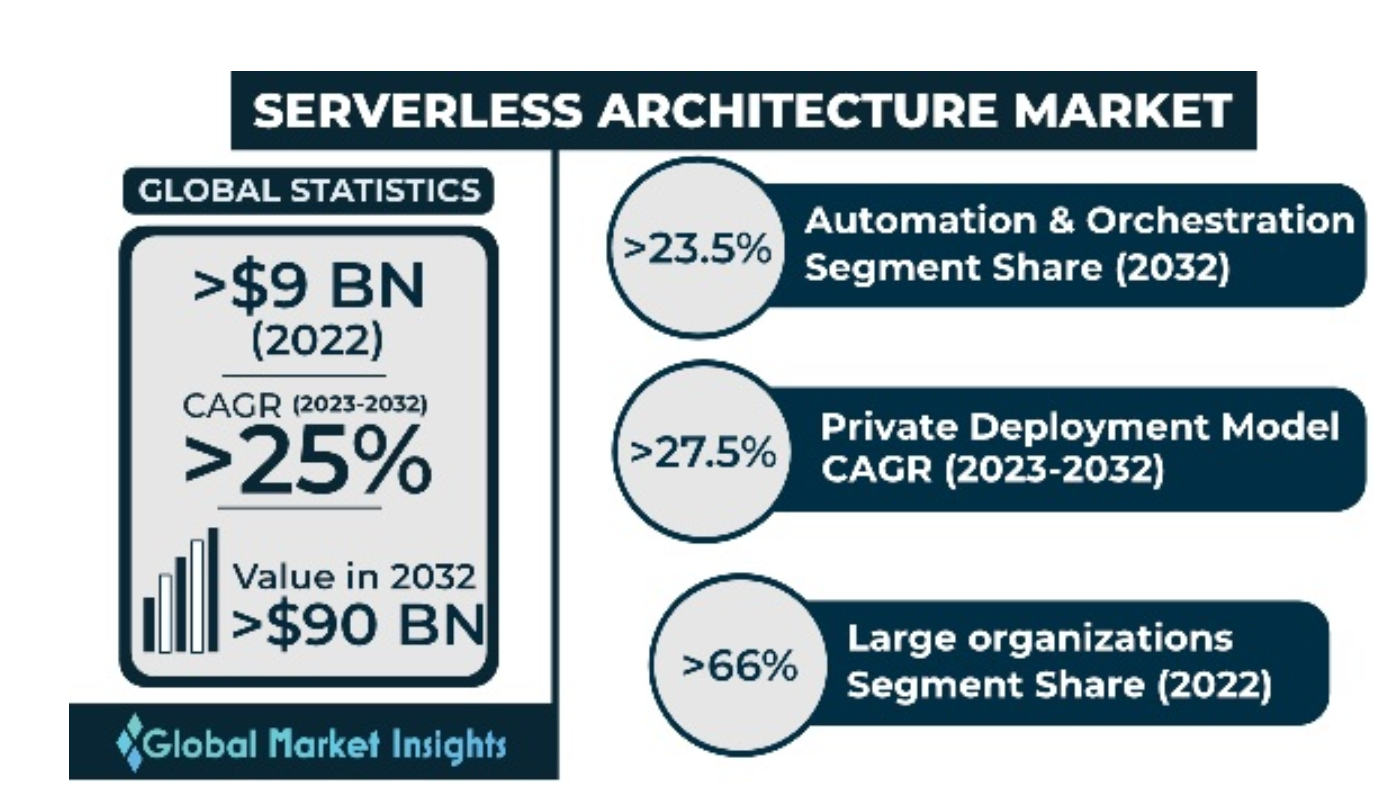
\includegraphics[width=0.5\linewidth]{images/Serverless-Arch-market.PNG}
    \caption{Serverless Global Market Share}
    \label{Serverless_global_market_share}
    (Ref: \cite{GMI_3796_2022} )
\end{figure}

\pagebreak

\section{Serverless Framework}
\subsection{FAAS: Function As A Service}
\par
\justifying
Function as a Service or \gls{FAAS} is the basic building block of Serverless framework, (including AWS Lambda or Azure Function). 
\begin{quote}
\begin{flushleft}
\textit{Function as a service is a category of cloud computing services that provides a platform allowing customers to develop, run, and manage application functionalities without the complexity of building and maintaining the infrastructure typically associated with developing and launching an app.}
\hfill \break
(\cite{Wiki_function_as_a_service})
\end{flushleft}
\end{quote}

\par
\begin{flushleft}
In \gls{FAAS}, the cloud vendors are responsible for providing and managing the complexity of related application server, infrastructure, frameworks, security, and everything that the application needs to execute a specific function in an application. 

\begin{quote}
\textit{
The “compute containers” executing your functions are ephemeral, with the \gls{FAAS} provider creating and destroying them purely driven by runtime need. Most importantly, with \gls{FAAS} the vendor handles all underlying resource provisioning and allocation—no cluster or VM management is required by the user at all.}\\ ( \cite{Roberts_Mike_2018} )
\end{quote}

Following \gls{FAAS} approach, Serverless offers on-demand functionality, which might live just for a single invocation. The cloud infrastructure will scale it to zero in preserve infrastructure and running costs. As such \gls{FAAS} functionalities are opinionated stateless applications. This is a key difference between other architectural cloud-based offerings like containers and PaaS. 
 \gls{AWS} Lambda is the first publicly cloud-based offering of \gls{FAAS} or Serverless. 

\subsection{Functional Triggers}
\gls{FAAS} functionalities are typically triggered by events. Event Types are defined by the vendors. The vendors for Serverless are also responsible in managing connections from various message sources. For Example:  Azure Functions can react to Messaging Sources like Event-Grid, Event-Hub, Blob Storage or simple \gls{HTTP} triggers. This approach fits perfectly with Microservices patterns of keeping the application event-driven and asynchronous.

One important feature of Functional Trigger, offered by Serverless, is that the developers do not need to write any infrastructure or platform-related code in this application. The Serverless framework also manages the consumption of data and its conversion to the “Cloud Event” format.

\gls{FAAS}, will not require any application server to up in running, it can be “Scaled to Zero” if there is no event triggered. This difference, as stated earlier my Mark Roberts, becomes a key factor in making \gls{FAAS} solutions cost-effective. \gls{FAAS} applications are booted and scaled up when an event is triggered from a configured event source.

However, the initial request in \gls{FAAS} has higher latency, (could be up to seconds,) than any other application platform. This “Cold restart” is an issue for \gls{FAAS} and for Serverless offerings. The restart will depend on many factors, predominantly the application runtime and its runtime libraries. The effect of “cold restart” on the Quality of Service depends on type of traffic and applications. 

\subsection{Vendor Locking}
In cloud computing, the \textit{"vendor lock-in"} is a major problem. When an organization adopts a specific cloud vendor, the migration of application and data to alternative providers becomes extremely difficult and highly expensive. The cloud vendor's framework and their adoption in application makes it incompatible with other vendors.
 The \textit{Vendor Lock-in} occurs in various ways: 
 \begin{itemize}
     \item by design: System design which is incompatible with software developed by other vendors.
     \item by using Closed architectures: Software developed using proprietary standards and  architectures that lacks interoperability with other applications by other vendors.
     \item by licensing: Software is licensed under under exclusive, non-flexible conditions.
 \end{itemize}

 Vendor lock-in discourages organizations in adopting new and emerging cloud technologies like Serverless. There is no standardization of Serverless design, data structure and code that could favour an easy transition from one cloud vendor to other, without an expensive redesign of the entire application. 

 \begin{quote}
 \textit{
Existing cloud computing solutions for enterprises have not been built with interoperability and portability in mind, hence applications are usually restricted to a particular enterprise's cloud or a cloud service provider.}  
( \cite{Opara-Martins-2014} )
\end{quote}
\par 
Existing cloud technologies, offered by proprietary vendors, are designed to work with specific technologies, which can limit the ability of customers to switch between different cloud providers.
\\
This leads to a \textit{"vendor lock-in"} to specific provider and their technology. This  situation can be problematic for businesses that want to maintain flexibility and avoid being tied to a single provider.
\end{flushleft}
\section{Cloud Native approach for Serverless}
\begin{flushleft}
Cloud Native Computing Foundation (\gls{CNCF}) introduced Kubernetes to counter vendor lock-in issues created by cloud vendors offering \gls{PAAS}. Kubernetes is a new platform allowing containerized applications to run in their own sandbox (\gls{POD}), isolated in their namespace.
Kubernetes is now accepted as the standard for \gls{PAAS}. All major cloud vendors support the deployment of Kubernetes clusters in their cloud environments
\end{flushleft}
\section{Knative }
\begin{flushleft}
The knative project was started by Google in 2018, with the aim to facilitate the deployment of a Serverless application using Kubernetes. Knative offers Serverless features like Scale to Zero, auto scalability, abstraction from \gls{PAAS} and Infrastructure, and use of the eventing framework.
Knative, leveraging from the underlying Kubernetes platform, offers a portable runtime and open API, which makes Serverless applications fully Cloud Native. This increases interoperability and eases the transfer of applications from existing cloud providers to others.
\begin{quote}
    \textit{Knative is an open-source initiative aiming to provide a platform for developing container applications on top of the Kubernetes container orchestration platform. It offers ready-to-use components built with Kubernetes Custom Resource Definitions (\gls{CRD}s) for developers to build, deploy, and scale their functions end-to-end from source code.} ( \cite{lin2019mitigating} )
\end{quote}

\subsection{Knative Function}
Knative provides the framework for creating a Cloud Native Serverless function that is deployed to a Kubernetes cluster. There are three components to Knative (a) Build, (b) Serving, (c) Eventing.

\textbf{Knative Build} component is responsible for converting the functional code to a container image, burning code or logic, the runtime, dependencies, configuration, and environment variable, etc. to \gls{OCI} standard Image, pushing it to an internal Kubernetes registry.
\begin{figure}[h]
    \centering
    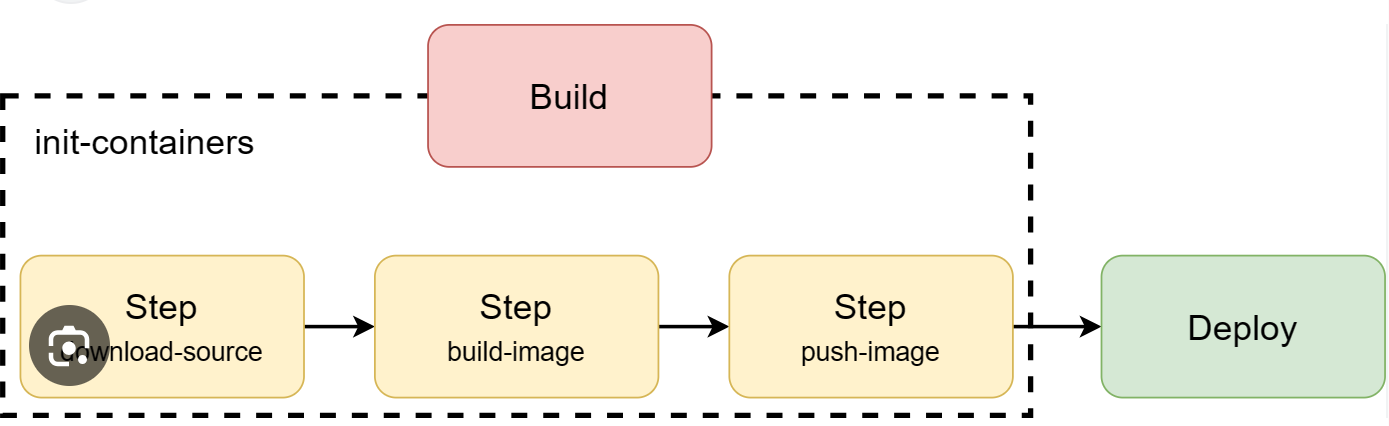
\includegraphics[width=0.5\linewidth]{images/knative-build.png}
    \caption{Knative Build Stage}
    \label{Knative_build_stage}
\end{figure}

\textbf{Knative Serving} is a request-driven provisioning component, responsible for auto-scaling Serverless containerized instances. It also takes care of load balancing. 
Knative Serving also abstracts the Kubernetes service to administer the provisioning of new service versions. It also manages configuration updates, by rolling out a new immutable revision representing the updated functional state. Each service saves specific routing information to redirect traffic to a specific instance version.
\begin{quote}
   \textit{Knative Serving is ideal for running your application services inside Kubernetes by providing a more simplified deployment syntax with automated scale-to-zero and scale-out based on \gls{HTTP} load. The Knative platform will manage your service’s deployments, revisions, networking, and scaling.} ( \cite{Sutter_Sampath_2020} )
\end{quote}
\par
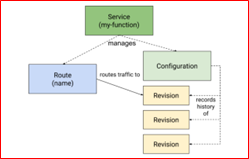
\includegraphics[]{images/knative-serving.png}

\subsection{Leveraging Service Mesh}
Knative leverage the service mesh to efficiently manage traffic routing between services which maintain immutable revision of Serverless application. It aids in satisfying the Serverless framework requirement of dynamic scaling, scale to zero and ease of deploying new versions. Various Service Mesh technologies are available that can be used in Knative example: Istio, kourier, etc.

\subsection{Knative Eventing}
Knative Eventing provides sets of primitives for consuming and producing events, assisting in satisfying the Serverless requirement of event-driven applications. 

\begin{quote}
\textit{Knative Eventing was to enable late binding of producers and consumers. It should be possible to connect consumers to producers without either component needing to know the configuration of the other.}
\end{quote}
\begin{flushright}
\cite{cncf_to_host_cloudevents_in_the_sandbox_2023}
\end{flushright}
 \hfill\break   
Just like any other message-driven system, the Knative Eventing component is composed of:
\begin{itemize}
    \item an Event-Source, which produces events from various sources.
    \item a Channel, which saves and buffers the event between and producers and consumers.
    \item 	and Subscriptions, which forwards events from Channel to services or other channels
\end{itemize}
\begin{quote}
\begin{figure}[h]
    \centering
    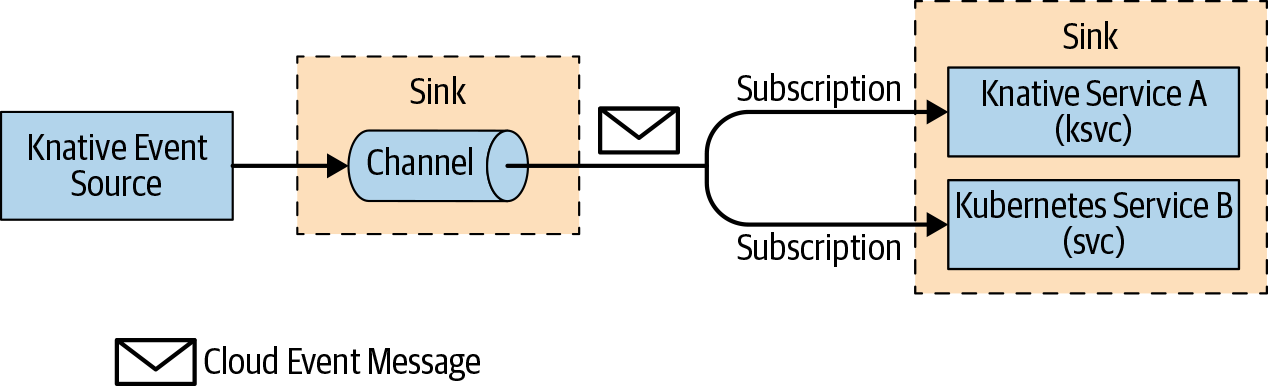
\includegraphics[width=0.5\linewidth]{images/knative-event-channel.png}
    \caption{Knative Eventing Channel,  Ref: \cite{Sutter_Sampath_2020}}
    \end{figure}
\end{quote}

The message-driven approach makes services loosely coupled and independent. Knative eventing framework makes Serverless applications event-driven and asynchronous. Knative being open source also allows the plugging of third-party Event Sources like Kafka Topics. 
\subsubsection{Using Broker and Triggers}
\textbf{Brokers} \break
Knative also offers Broker, which are Kubernetes Custom Resources and services, defining the event mesh, collecting pool of events. Knative Eventing will implicitly create a Knative Eventing Channel for the Broker. The Brokers expose an endpoint, using ingress. Event Producers can POST event directly to broker using the ingress based endpoint.
\hfil \break
\textbf{Triggers} \break
The Custom resources for Knative Eventing, also includes Triggers, which is responsible to send events to a configured \textit{Event Sinks}. Triggers subscribe to Broker's underlying event channel, consuming events as they arrive.\\
The downstream Sink service, supports a CloudEvent response, which is routed back to the Broker, and finally to event channel.
\hfill \break
\textbf{Filters} \break
Knative Broker also supports event filtering.
\begin{quote}
    \textit{
    "Event filtering is a method that allows the Subscribers to show an interest in a certain set of messages that flows into the Broker."
    ( \cite{Sutter_Sampath_2020} )
    }
\end{quote}
Trigger is also responsible for Filtering of events before dispatching it to configured Sink. It subscribes to the broker to consume events, then apply filter on it.


\begin{figure}[h]
    \centering
    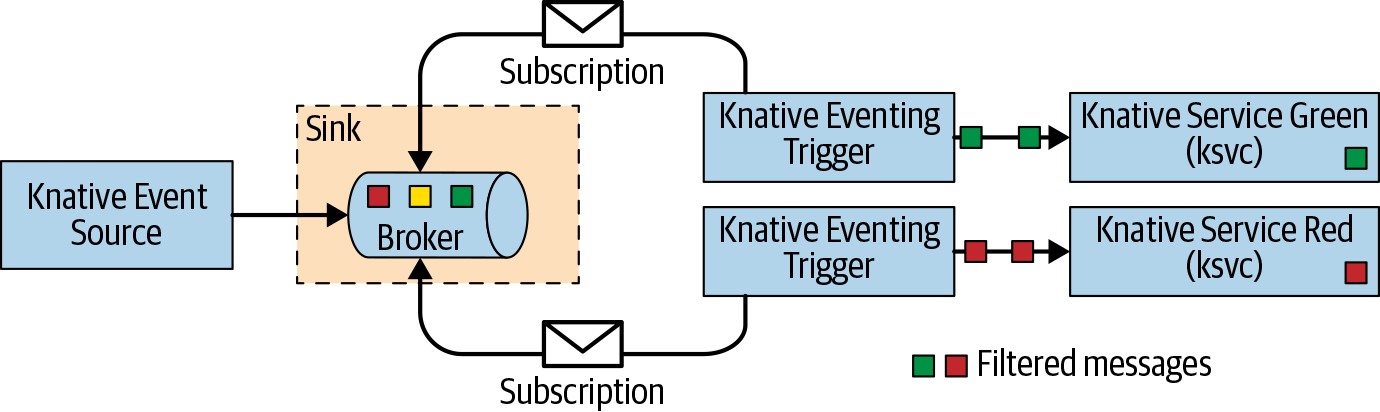
\includegraphics[width=1.00\linewidth]{images/knative-event-broker.png}
    \caption{Knative Event Source, Broker Trigger and Sink}
    \begin{quote}
    \textit{"The filters are applied on the CloudEvent attributes of the messages, before delivering the message to the interested Sink Services" \\ (  Ref : \cite{Sutter_Sampath_2020} ) }
    \end{quote}
\end{figure}
In the easiest term, Knative Broker is an abstraction over event channel, subscription and triggers.

\par
The developers leverage for Knative API and Eventing platform to consume events in their functional code without writing any infrastructure code for consuming and parsing it. The API makes it possible to consume events in the standard “CloudEvent” format.
\end{flushleft}
\pagebreak
\section{Azure Function}
\begin{flushleft}
\textbf{Azure Function} is a Serverless offering by Microsoft. It allows developers to deploy their \gls{FAAS} application on Azure Cloud using a Pay-as-you-go model. It followed all the features of Serverless, like the scale to zero, horizontal scalability, complete abstraction from the Platform, and eventing framework. It offers \gls{SDK} and \gls{CLI} to build and Deploy Serverless applications to the cloud, using various programming languages and frameworks like Java, .Net, NodeJS, etc.

Azure Functions adopts the Azure Eventing framework to provide a comprehensive set of event-driven triggers and bindings. This binding connects Azure functions to other services without having to write extra code, providing the capability of Azure function to be asynchronous and event-driven.

Azure Serverless Functions are grouped in \textit{Azure Function App}, which provide convenience in deployment, management, configuration, scalability and resource sharing, represented as one logical unit. 
Azure deploys its Serverless code, runtime dependencies and configuration information under its \textit{Functional App}'s file storage. 
\end{flushleft}
\pagebreak
\section{Azure Eventing}
\begin{flushleft}
Azure Functions leverages Azure eventing framework to create Event-Driven, Asynchronous Serverless Functions. The common use case for this feature is creating Workflow. 
\begin{quote}
    \textit{Serverless is a great fit for event-driven architectures because each message acts an individual independent unit of work that can be processed Serverlessly.} \cite{ANDERSON_2024}
\end{quote}

Azure Eventing framework supports event-sourcing and event-subscription. It consumes events from the Eventing Channel, triggers, and routes it to the Functional instances. If the instance is scaled to Zero, a new instance is started. Azure Serverless framework abstracts all infrastructure and platform complexity from the code, making the function API consume CloudEvent formatted data. The configuration also allows the Azure function to push data back to the Event Channel.

\subsubsection{Three Patterns of Knative Eventing}
\begin{itemize}
    \item Source To Sink: It is a very basic connection between the Event Source to service that receives the event unconditionally (or SINK). There is no support for filtering, queuing, etc.

    \item	Channel and Subscription: Knative defines a Channel and subscribes it to other back-end messaging services like In-Memory, Kafka, etc. for event sourcing. Each message in the channel is in Cloud-Events format. There is no message filtering in the Channel.

    \item Triggers and Broker: Knative provide a Broker which is an abstraction over underlying Event Channel and Event Triggers. Trigger is responsible for subscription and filtering of events, based on Cloud-Events attributes. Triggers configures a Sink, which is the destination endpoint for the filtered events. 
\end{itemize}
\end{flushleft}

\section{CloudEvents}
\begin{flushleft}
CloudEvents is a common data format or schema to defining "events". It aims to provide interoperability across various cloud platform and services. It is an Open-source and maintained by \gls{CNCF} Serverless working Group.
\par
\begin{quote}
    \textit{CloudEvents, an industry initiative that members of the \gls{CNCF} Serverless Working Group contribute to, provides a consistent set of metadata to make events easier to work with for publishers, middleware, subscribers, and applications.}
    \newline ( \cite{cncf_to_host_cloudevents_in_the_sandbox_2023} )
\end{quote}
\par
CloudEvents at its core, defines a set of \textit{metadata}, which holds minimal information that can be used to route events. It also supports batching of multiple events in a single API calls. One of the major goal of CloudEvents is to increase interoperability and keep both event producer and consumer decoupled. This is achieved by prohibiting the routing, authorization, integrity and confidentiality information from the message format. This facilitates re-delivery of events or delivery over complex distributed or multi channel system.
\par
CloudEvents supports events in \gls{JSON} format and support \gls{HTTP} protocol binding. A \gls{JSON} formatted CloudEvents , transported over \gls{HTTP}, uses a "media type" \textit{application/cloudevents+json}. The CloudEvents specification using \gls{JSON} formatting defines set of mandatory attributes. The two important attributes which is a key for Cloud-Native eventing is \textbf{type} and \textbf{data}.
\newline
\textbf{A sample CloudEvents:} 
\begin{verbatim}
[
  {
    "id": "b3ccc7e3-c1cb-49bf-b7c8-0d4e60990119",
    "source": "/postman/cloudevent/azure/test",
    "specversion": "1.0",
    "data": {
      "custID": "44458111",
      "amount": 52200
    },
    "type": "InvoiceGenRequest",
    "time": "2023-10-28T21:36:00.147165Z"
  }
]
\end{verbatim}
The attribute \textbf{data}, represents the application data object, that is transported across different applications. The data is parsed by default \gls{JSON} parser. For parsing oher data formats an attribute \textbf{"datacontenttype"} is used. Most eventing framework provide their own event router, which are optimized to use any CloudEvent attribute like \textbf{type}.
\par
\gls{HTTP} protocols is used to transport CloudEvent, to any \gls{HTTP} supported endpoint, like RESTful web services, EventGrid, etc. Serverless framework, adopting CloudEvents,  parse the data before calling the Serverless function. Open-Source \gls{SDK} are also available to create CloudEvent data.
\pagebreak
\par
\textbf{Sample Curl Request to POST CloudEvent:}
\begin{verbatim}
curl POST 'https://eventmanagertopic.europe-1.eventgrid.azure.net/api/events' \
    --header 'Content-Type: application/cloudevents-batch+json;charset=utf-8' \
    --data '[
          {
            "id": "b3ccc7e3-c1cb-49bf-b7c8-0d4e60990119",
            "source": "/postman/cloudevent/azure/test",
            "specversion": "1.0",
            "data": {
              "custID": "44458111",
              "amount": 52200
            },
            "type": "InvoiceGenRequest",
            "time": "2023-10-28T21:36:00.147165Z"
          }
    ]'
\end{verbatim}
\end{flushleft}
\pagebreak
\section{Building and Deploying Serverless Function}

\subsection{Building and Deploying in Azure}
\begin{flushleft}
Azure \gls{SDK} and \gls{CLI} provide templates for creating Azure Functions, giving the choice of programming language and event schema.
\par
Azure \gls{CLI} archives and publishes the code to the File System under the Function App. The deployed Serverless function will remain in a dormant state (i.e. scaled to zero). The function performs a “Cold Start” when the event is called by Event Triggers.
\end{flushleft}
\subsubsection{Build Automation}
\begin{flushleft}
There are various option to achieve automation in deployment of Azure Serverless Functions. Source Control integration connects the Function App to a GIT Repository, which will trigger deployment whenever an updated code is committed and pushed. 
\end{flushleft}
\begin{figure}[h]
    \centering
    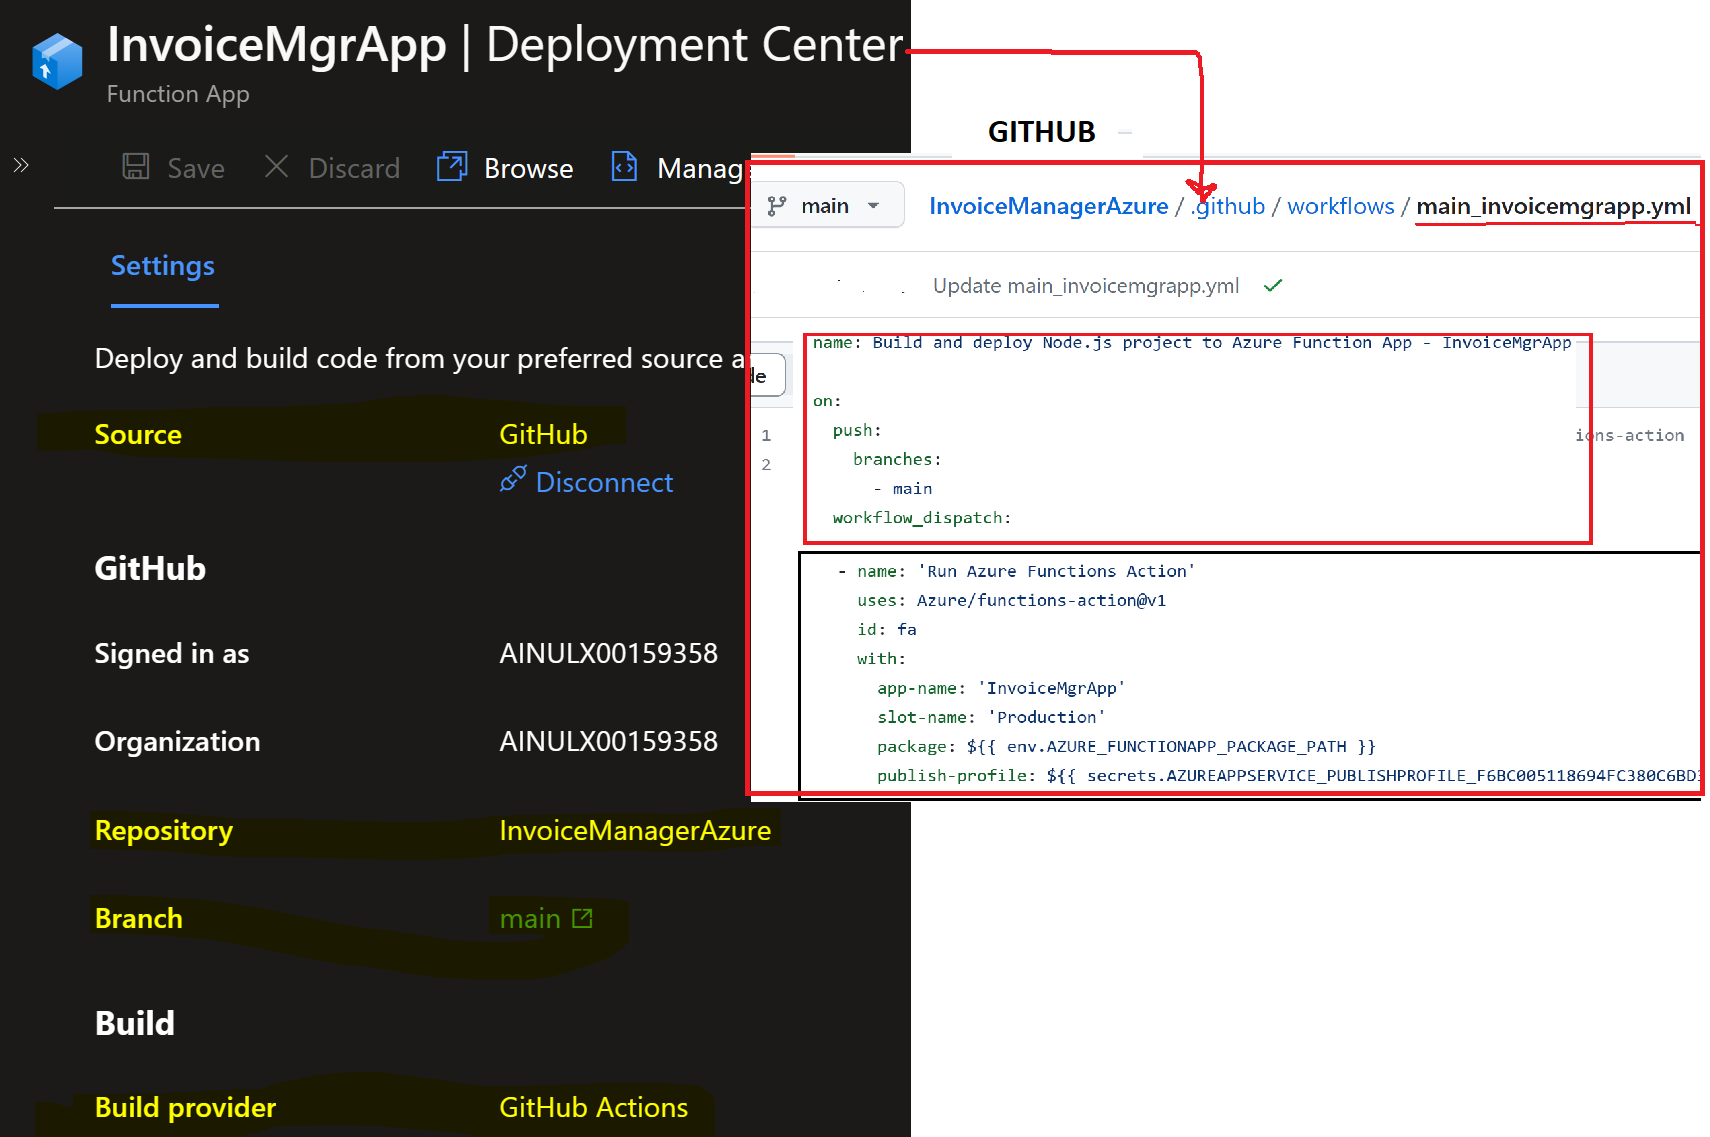
\includegraphics[scale=0.20]{images/AzureDeploymentCenter.PNG}
    \caption{Azure Deployment GitHub Workflow}
\end{figure}

\subsection{Build and Deployment in Knative}
\begin{flushleft}
The Knative \gls{CLI} offers a build utility which uses the project name and the image registry name to construct and push a fully qualified container image, in \gls{OCI} format, for the function.  
The container image has the application's language specific runtime and functional code.
\hfill\break
Knative Serving deploys the container image as Kubernetes application, pulling the image from registry for first pod initialization.
\par
\begin{verbatim}
# build Knative functional image and push it to docker repository
func build --registry docker.io/x00159358 \
           --image docker.io/x00159358/invoicemgrimg:latest \
           --push \
           --verbose
\end{verbatim}

\par
Azure function do not create a containerized image. Azure \gls{CLI} provide utility to package the artifacts and archive to Azure File Storage. Azure functional loads the application runtime and code into memory and executes it.

\end{flushleft}
\pagebreak
\section{Cold Start}

\quote{
Defining Cold Start : \\
\textit{This phenomenon is associated with a delay occurring in provision a runtime container to execute the functions.} \\ \cite{vahidinia2020cold}
}
\begin{flushleft}
\par
A cold start in Serverless refers to an increase in latency for Functions which haven’t been called recently. The Serverless framework will need to scale its instance from zero to one, before it can process the request. The cold start latency will be passed to request, which need to wait until an becomes fully ready to serve.
\par
 The startup delay is influenced by various factors including bootstrapping application runtime, Serverless code and its dependent libraries. This bootstrapping startup delay is also witnessed when Auto-Scalar provisions instances to support the traffic. This initialization time is unavoidable and lasts until the application starts responding. Depending on the application use case, this latency caused by Cold-start can create a request backlogs, which may eventually result in timeout.
\par
 Consider a traffic request bust of 3000 in 1 sec. If the cold start delay is 3 sec, there will be a backlog of nearly 9000 requests. Backlog will eventually get cleared after Serverless application is fully started. If the request timeout is 1 sec, nearly 80 percent of the request might be timed out.

\subsection{Azure Cold Start}
Azure Functions has a longer cold start time, because of its uses of a \textbf{Dynamic Provisioning Model}.

\begin{quote}
    \textit{Dynamic concurrency automatically determines optimal per trigger concurrency settings for your workloads and adjusts as your load patterns change over time.}    ( \cite{Cachai_Gailey_2022} )
\end{quote}
\par
In short, the function is only created and scaled when needed. This can lead to longer cold start times, especially for functions which is not called frequently.
\par
Serverless offering from cloud vendors like \gls{AWS} Lambda use Static Provisioning Model, which ensures that a minimum functional instance  are always running, reducing the cold start time even for less frequently called Functions.
\par
There are many factors which effect the latency of the cold start when using Cloud Vendors like Azure. Programming Runtime environment plays a significant role in Cold Start of Serverless functions.

The Research study titled "An Investigation of the Impact of Language Runtime on the Performance and Cost of
Serverless Functions", conducted series of tests and analysis measuring Cold and Warm Startup latency of \gls{AWS} and Azure Serverless functions, using NodeJS and DotNet runtimes. 

\begin{quote}
    Test was conducted using : \newline
     \textit{ " There were a total of 144 Cold-Start tests (for both runtimes) over a 6-day period. These were performed at the same 1-hour intervals as in \gls{AWS} Lambda testing. "} 
     \begin{flushright}
         ( \cite{8605773} )
     \end{flushright} 
\end{quote}

\hfill \break
\begin{figure}[h]
    \centering 
    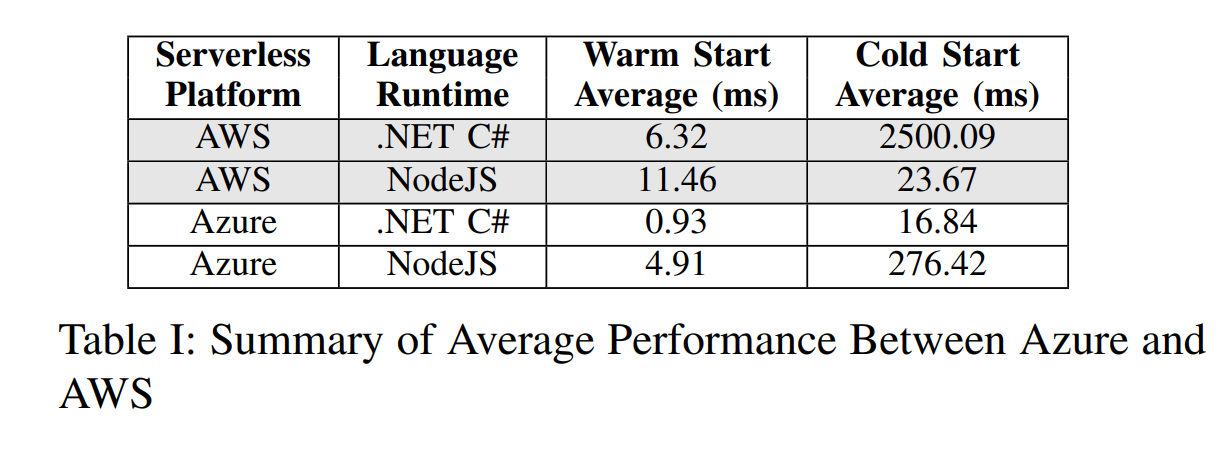
\includegraphics[width=0.5\linewidth]{images/Table_Ref_Code_Start_UCC-Companion.2018.00050.PNG}
    \caption{test result showing performance of Serverless startup} 
    \begin{flushright}
         ( \cite{8605773} )
    \end{flushright}
\end{figure}
\pagebreak
\subsection{Knative Cold Restart}
Knative Serving instructs the Kube API to provision the Serverless application, when it needs to scale up the instances. 

There are different distinct stages of execution leading to provisioning of the \gls{POD}. 
\newline
\textbf{Cold Start:} When the application is being started for the first time
\newline
\textbf{Warm Disk Start:} When the docker image is already cached. The process starts from mounting of image, starting the container, application runtime and pods
\newline
\textbf{Warm Memory Start:} The container is resumed from the paused state. The costly, time consuming process of image pull, mounting and starting of container is avoided, thus speeding up the startup time.
\newline
\textbf{Warm CPU start:} In this case the container is already running as such the only latency that will apply will be the time application takes to respond to the request. In this is a case application was not scaled to zero.
\pagebreak
\begin{figure}[h]
    \centering
    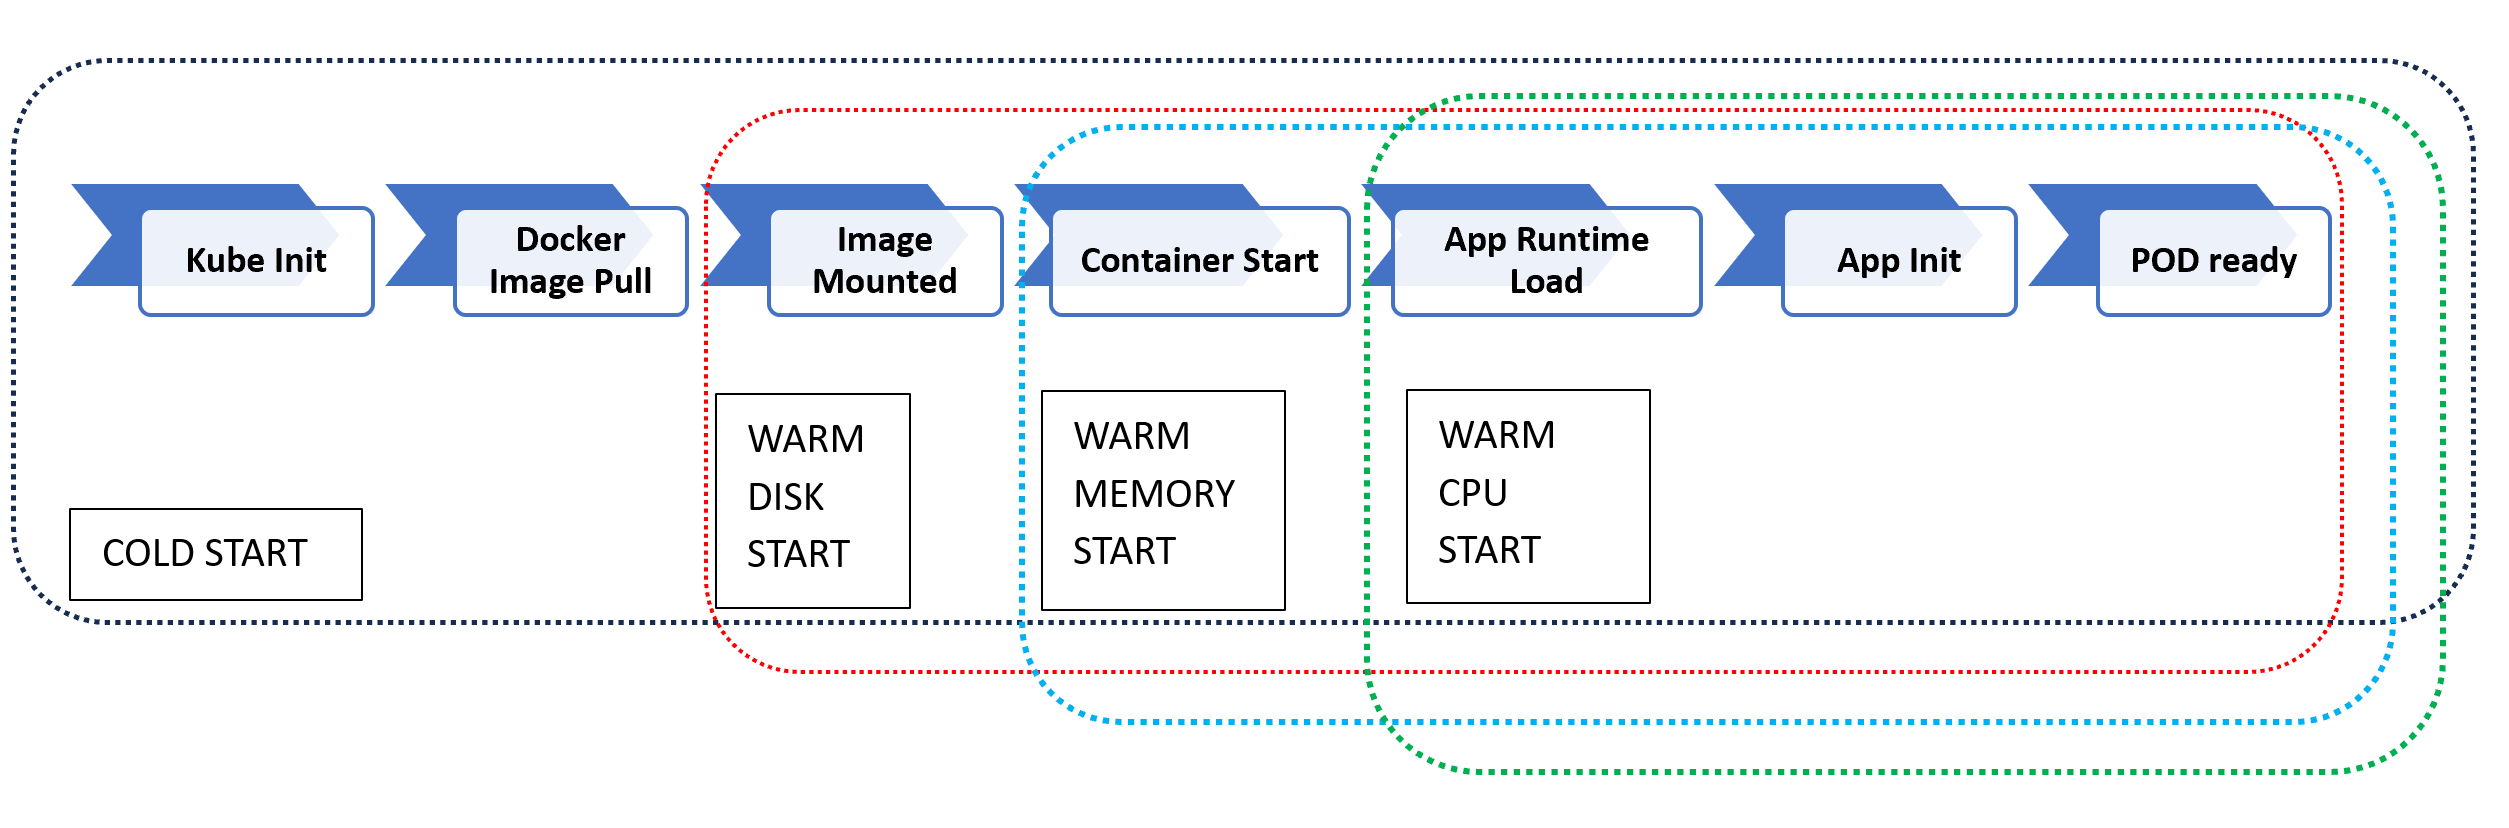
\includegraphics[width=1.0\linewidth]{images/Knative_lifecycle.PNG}
    \caption{Knative Lifecycle}
    \label{fig:enter-label}
\end{figure}
\par
\begin{figure}[h]
    \centering
    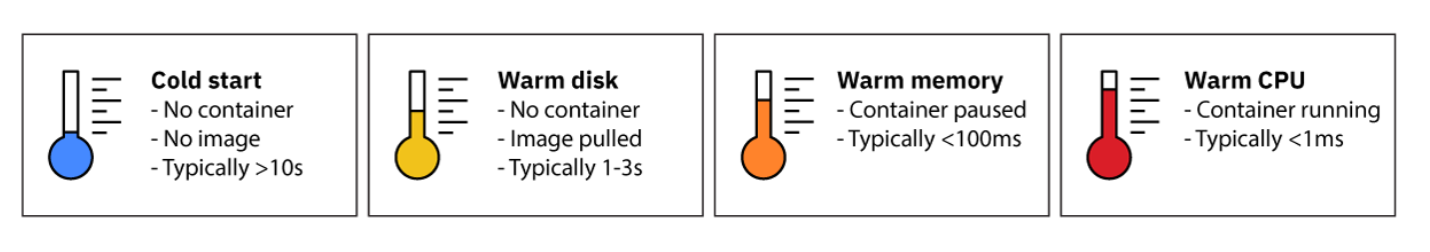
\includegraphics[width=1.0\linewidth]{images/ColdStart-Knative-Image.PNG}
    \caption{Knative Guage for Cold Start}
    \label{fig:enter-label}
\end{figure}
\par
\quote{
\textit{When a cold start or a warm disk start is used during a scale-from-zero, there is a noticeable delay between when a user makes a request and when the application responds to it, resulting in a poor user experience and possibly other consequences, such as missed service level objectives (SLOs). 
\hfill\break
In a worst-case scenario, when a cold start is used during a scale-from-zero, it is even possible to encounter client timeouts if the application doesn't respond in time.} \hfill\break ( \cite{Schweigert_Hadas_2022} )
}
\end{flushleft}
\pagebreak
\section{Mitigation to Cold startup}

\subsection{ Azure Mitigation to Cold startup}
\begin{flushleft}
Azure handles this issue by keeping a pool of server in a "warm state", and drawing these servers as "workers" from pool. At any point of time, there are servers in the pool which are idle and pre-configured with Configuration and Functional runtime in a ready and running state. This feature is only available in Azure's Premium Plan.
\end{flushleft}

When execution of function is triggered by incoming traffic:
\newline
Azure will allocate a pre-configured server from the pool. The server already has a functional runtime and configuration on it.
\newline
After allocation, the server re-configures the functional runtime based on the application requirements.
\newline
The Server now resets the Functional runtime and load any required extensions, using the \textit{function.json} file, specified the application manifest.
\newline
In the last stage the Function is now loaded into memory and executed. Time take to complete the last stage depends on language used, size of application etc. The function is now in a ready state serving request.
\par
\begin{flushright}    
\begin{quote}
    \textit{"Making these 'pre-warmed sites' happen has given us measurable improvements on our cold start times. Things are now on the order of three to four times faster" 
 - ( \cite{Understanding_serverless_cold_start_2018} } )
\end{quote}
 \end{flushright}

\begin{figure}[h]
    \centering
    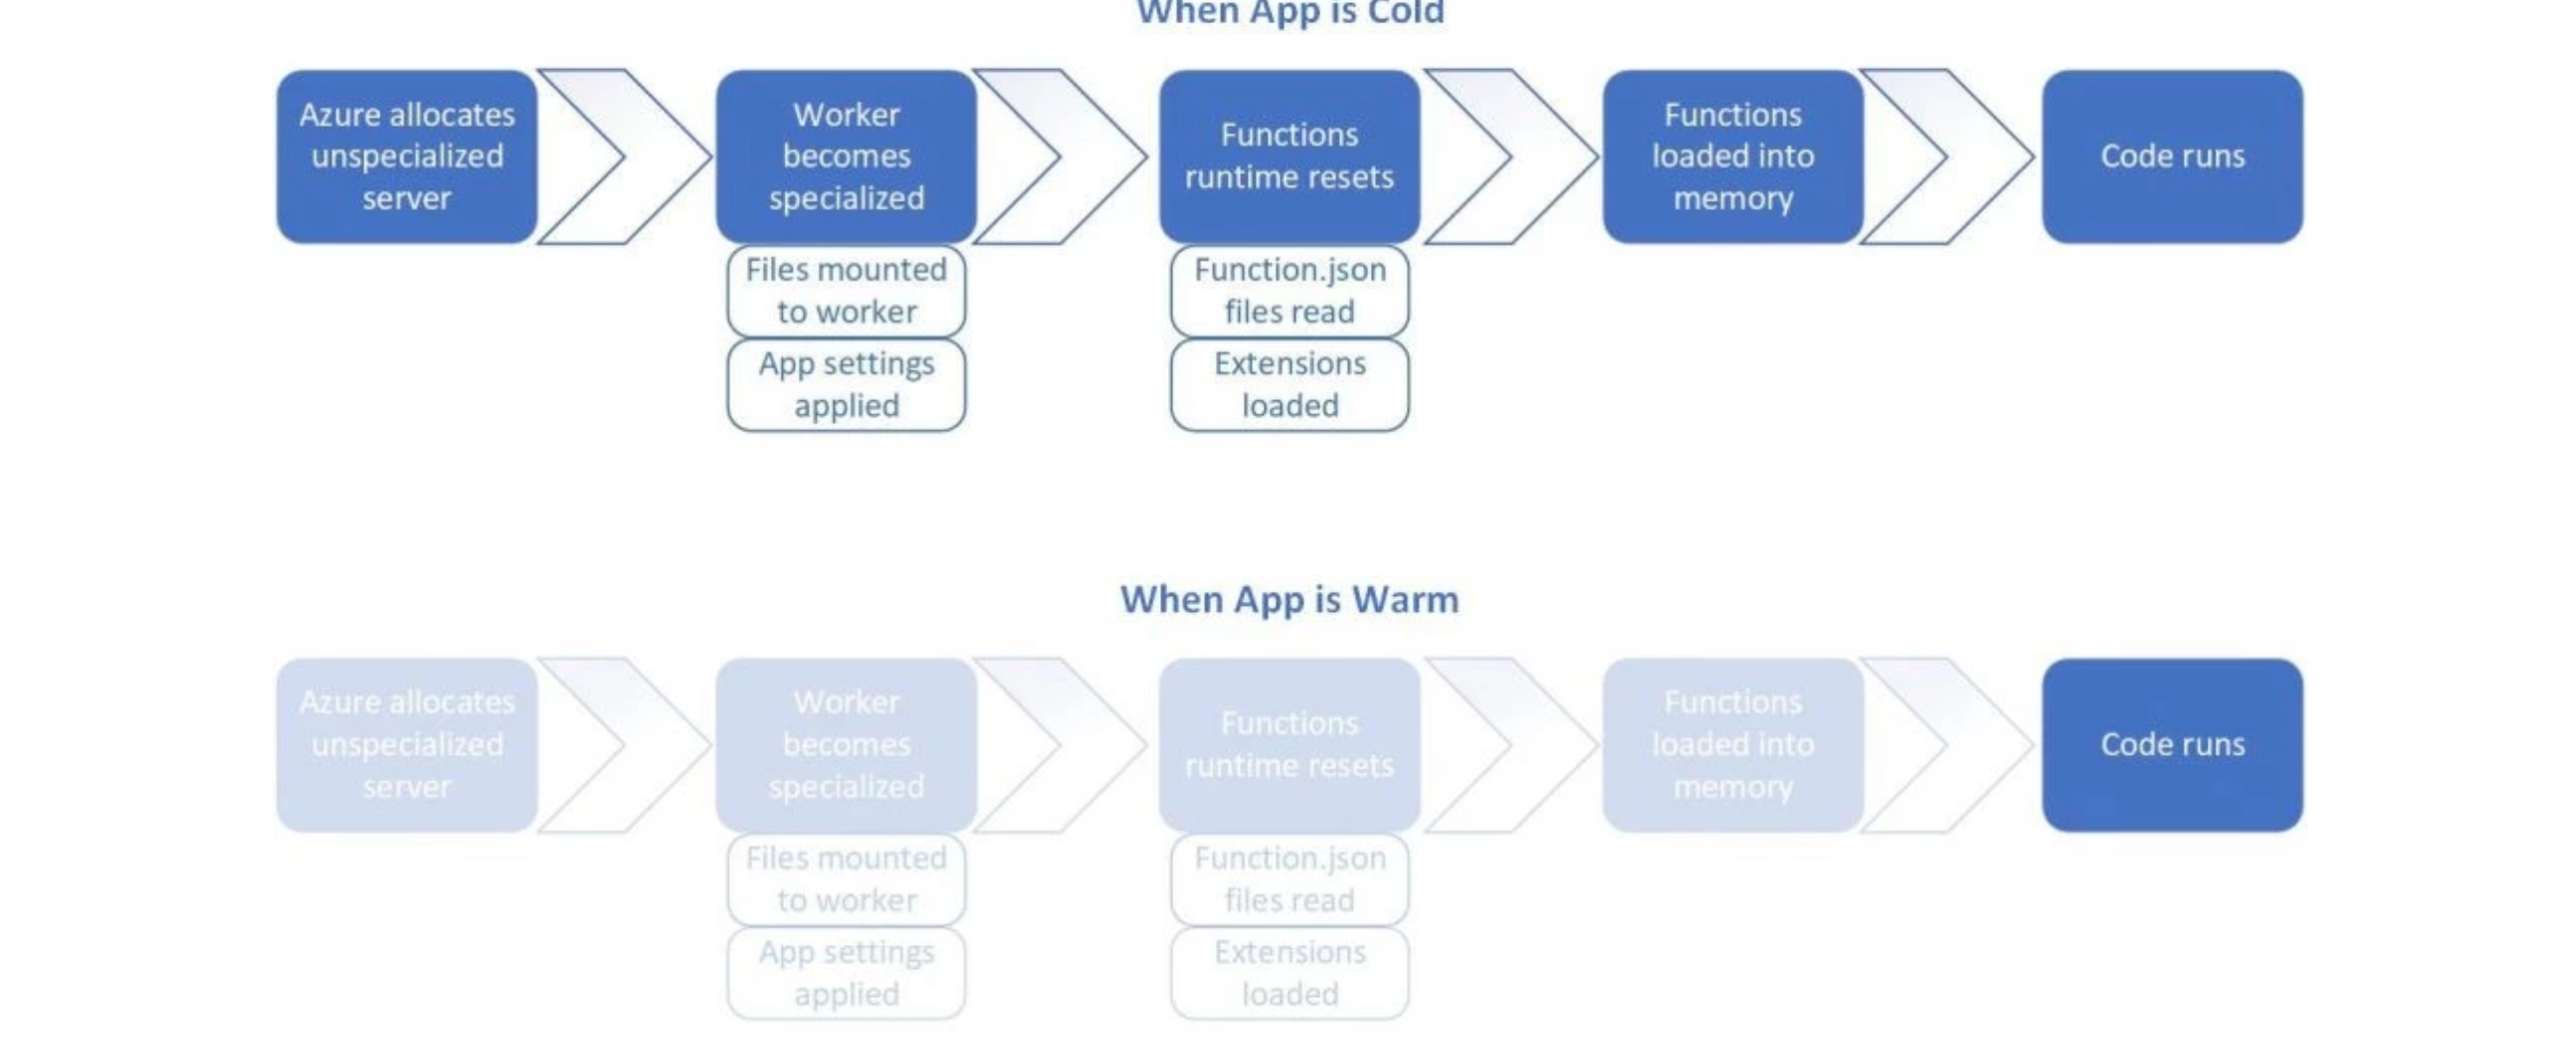
\includegraphics[width=1.0\linewidth]{images/Azure_lifecycle.PNG}
    \caption{Azure Lifecycle}
        Ref: \cite{Understanding_serverless_cold_start_2018}
\end{figure}

\pagebreak
\subsection{ Knative Mitigation to Cold startup latency}
\begin{flushleft}
There are a number of ways to reduce Cold Stat-up Latency ( scale from zero latency).
\newline
\begin{itemize}
    \item Choose better Runtime and programming language : Some programming language are faster to startup, while other have extra overheads. Optimized runtime can reduce startup time. Java runtime has higher initialization time than other programming languages. As such choosing correct programming languages will contribute in lowering down Cold-Startup time.

    \begin{figure}[h]
        \centering
        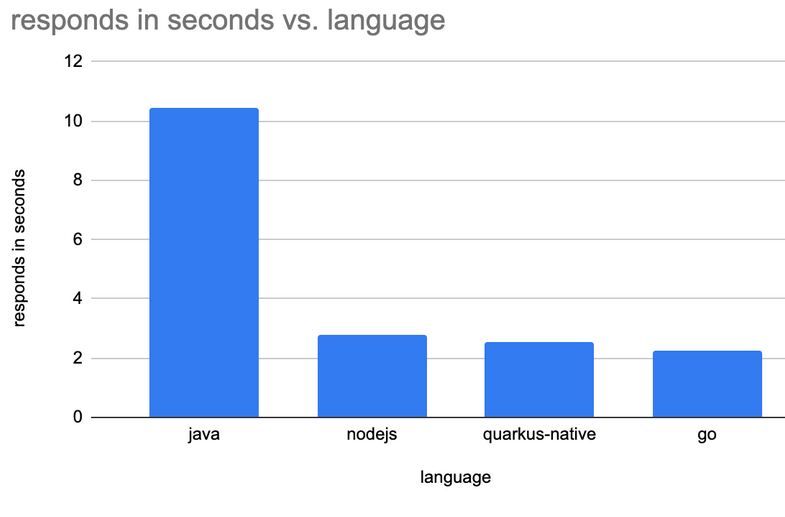
\includegraphics[scale=1.0]{images/Knative_app_runtime_startup.PNG}
        \caption{Knative App Runtime Startup}
            Ref: \cite{Schweigert_Hadas_2022}
        \end{figure}
    \item Speedup image pull. Image Pull effects initial Cold Startup time,because of network latency in downloading container image from repository. 
    \begin{itemize}
        \item Use small size of Base image e.g. "alpine base image".
        \item Keep dependencies and additional libraries to base image to bare minimum.
        \item Use Stratergy to do a lazy pull of image
        \item Avoid \gls{POD}'s image pull policy as "Always"
        \item Use specific image digest rather than using the latest tag
        \item Cache image to all nodes.
        \item try pull image to Kubernetes docker registry through different deployment channel
    \end{itemize}
    \item Avoid Cold-startup completely: Keep at-least one container to be always in a running state. This can be adjusted using deployment flag \textit{"min-scale"} to 1. But this options destroys the basis if Serverless concept, where application should be scaled to zero if there is no traffic.
    \item Reduce the frequency of your application scaling down
    The deployment flag \textit{"scale-down-delay"}, causes increase the time window before Knative service decides to scale down the container.
    \item retention period for Scale to zero, increases minimum amount of time for the last pod to remain after a scale-to-zero decision has been made. This is controlled by the deployment flag \textit{"scale-to-zero-pod-retention-period"}.
\end{itemize}
\end{flushleft}
\pagebreak
\section{Autoscaling in Knative}
Figure ~\ref{Knative Service Architecture} explains the full process of Autoscaling in Knative Serving Infrastructure.
\quote{
\begin{figure}[h]
    \centering
    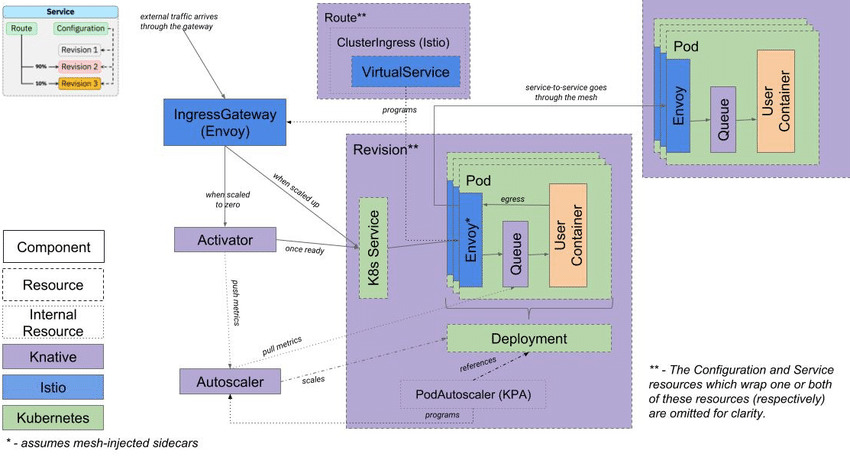
\includegraphics[width=1.0\linewidth]{images/Knative-Serving-Architecture.jpg}
    \caption{Knative Service Architecture }
    \cite{Towards_Serverless_as_Commodity}
    \label{Knative Service Architecture}
\end{figure}
}
\begin{flushleft}
The interesting case is when scaling from Zero to One:
\begin{itemize}
\item  Traffic comes to Ingress Gateway, then to the Serverless Services.
\item since the Pods are scaled to zero, requests are routed to the Activator. (i.e. Inactive Case).
\item Activator passes metrics to Autoscaler which obliged for scaling up the Pods, (from zero to 1).
\item Activator calls Knative Serving Deployment to spin up a pod, with all its containers and sidecars. 
\item \gls{POD}'s cluster IP is now updated in Serverless Services.
\item Once Pods are scaled above zero, Serverless Services updates the Route, disconnecting the Autoscaler. The traffic is now routed directly to \gls{POD}'s service Proxy.
\item The Knative \gls{POD}'s sidecars and Envoy provide metrics which is now scared to Autoscaler directly, so that it can now decide to need to scale further based on incoming traffic.
\end{itemize}
\end{flushleft}
\begin{quote}
    \begin{figure}[h]
    \centering
    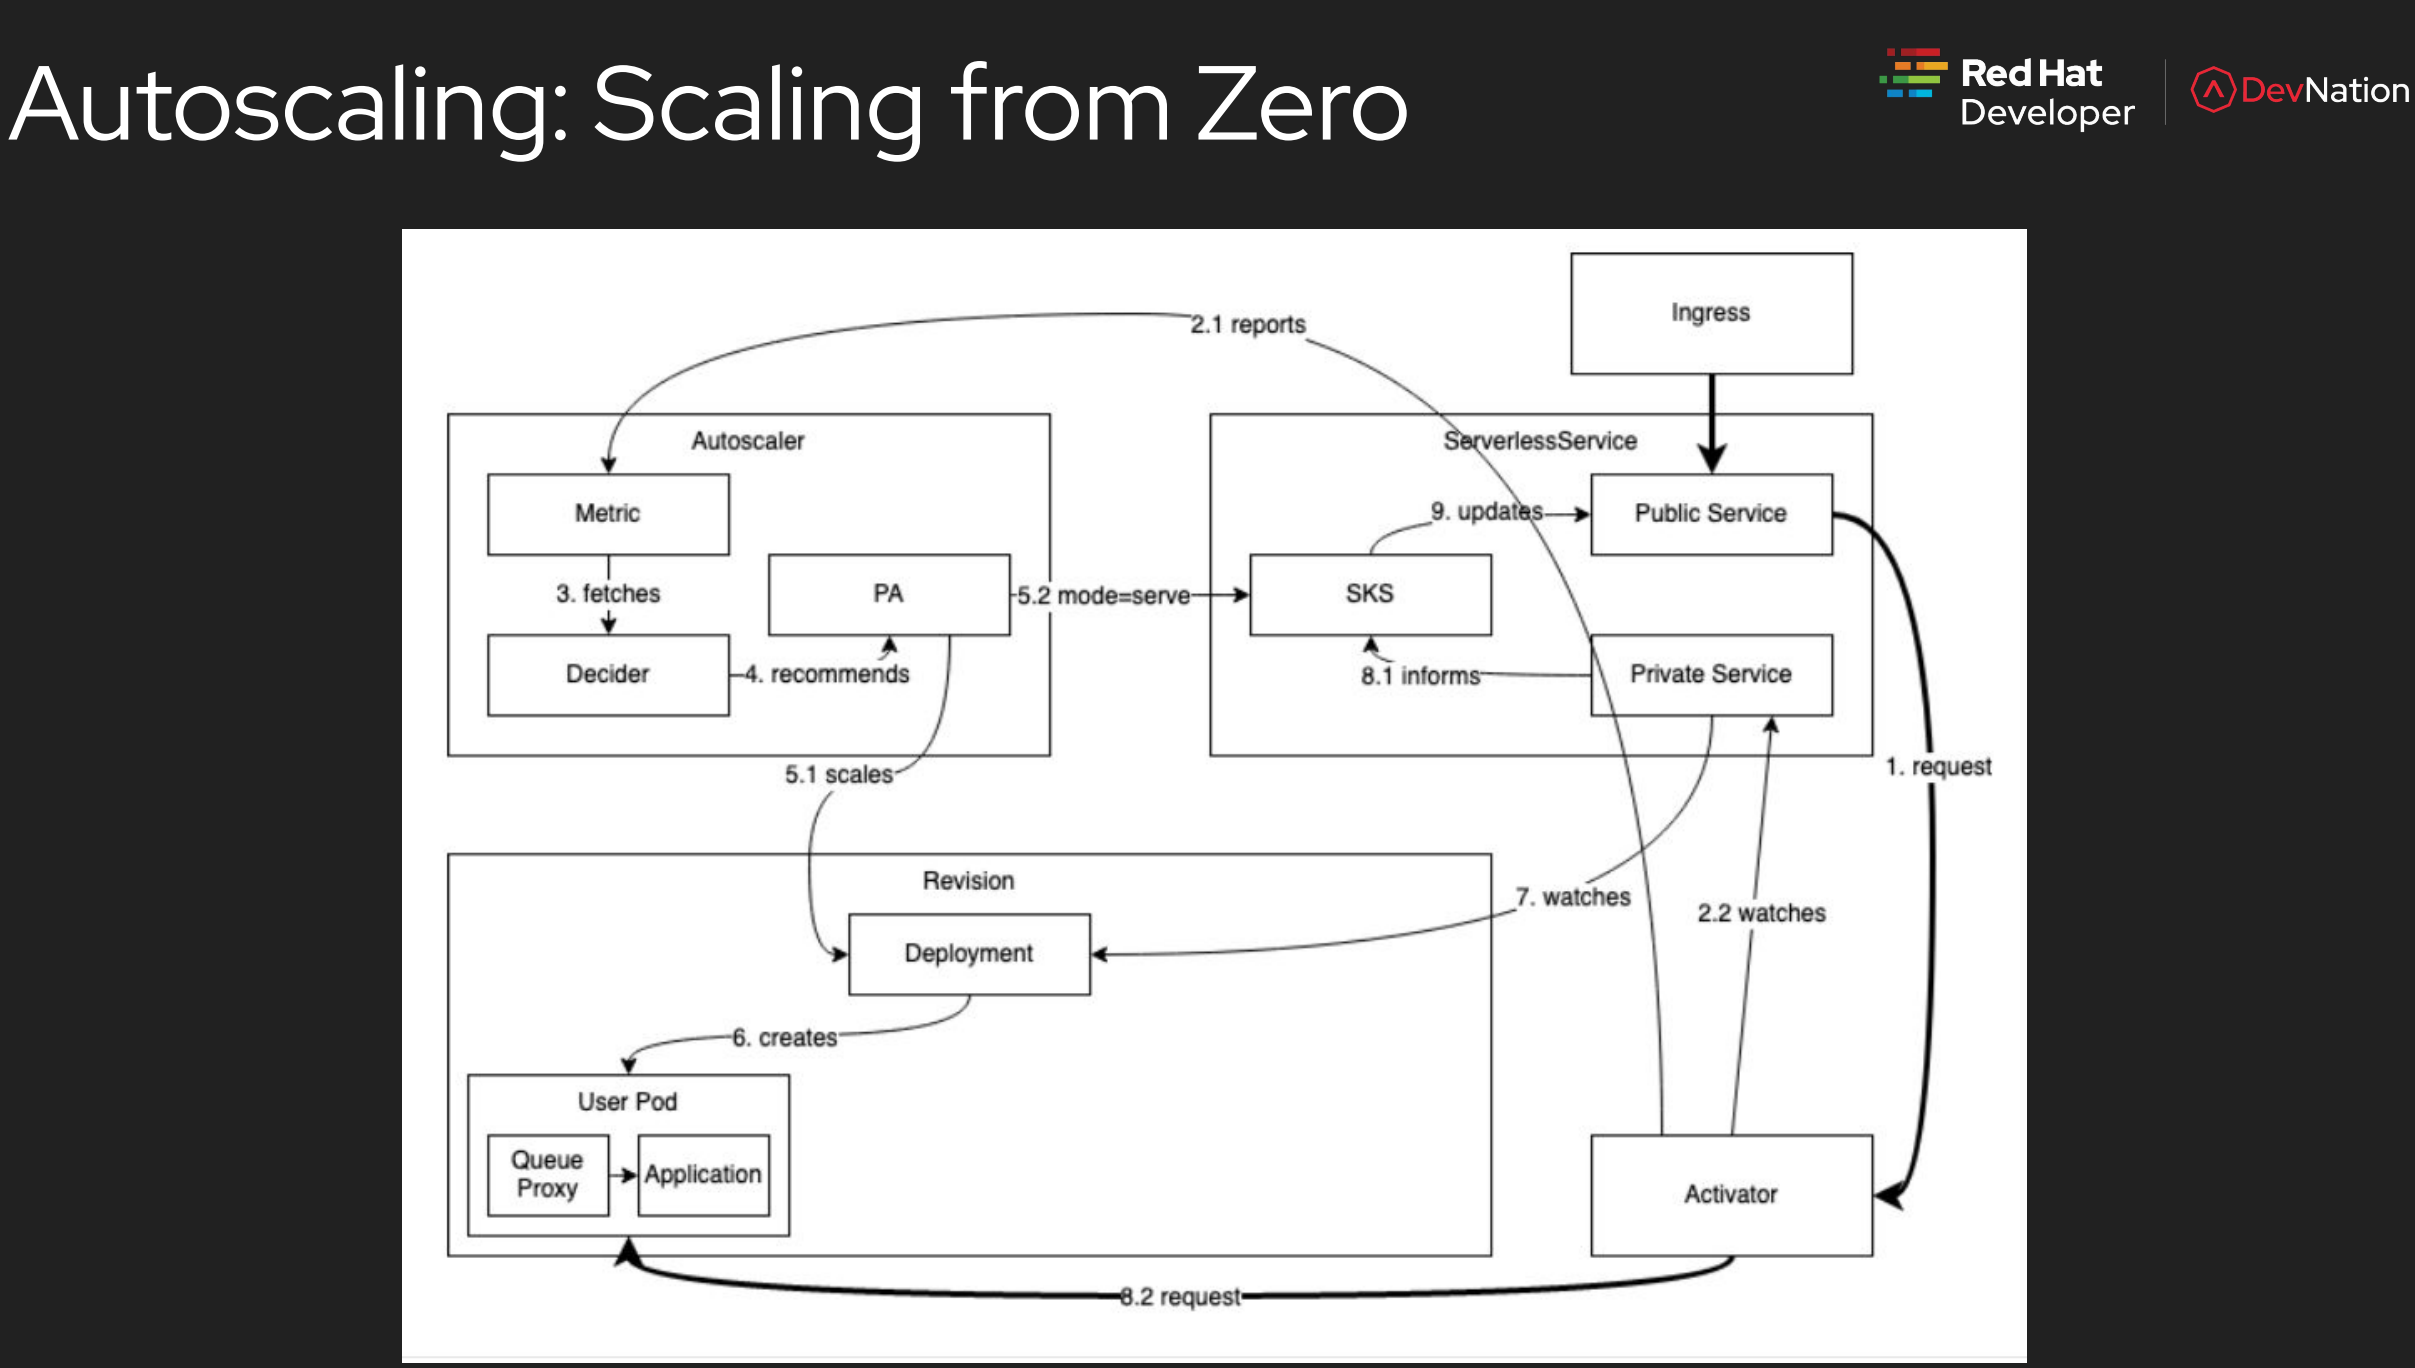
\includegraphics[width=0.5\linewidth]
    {images/KnativeAutoscaler-1.PNG}
    \caption{Autoscaler : Cold Start Case, Zero to One}
\end{figure}
\begin{figure}[h]
    \centering
    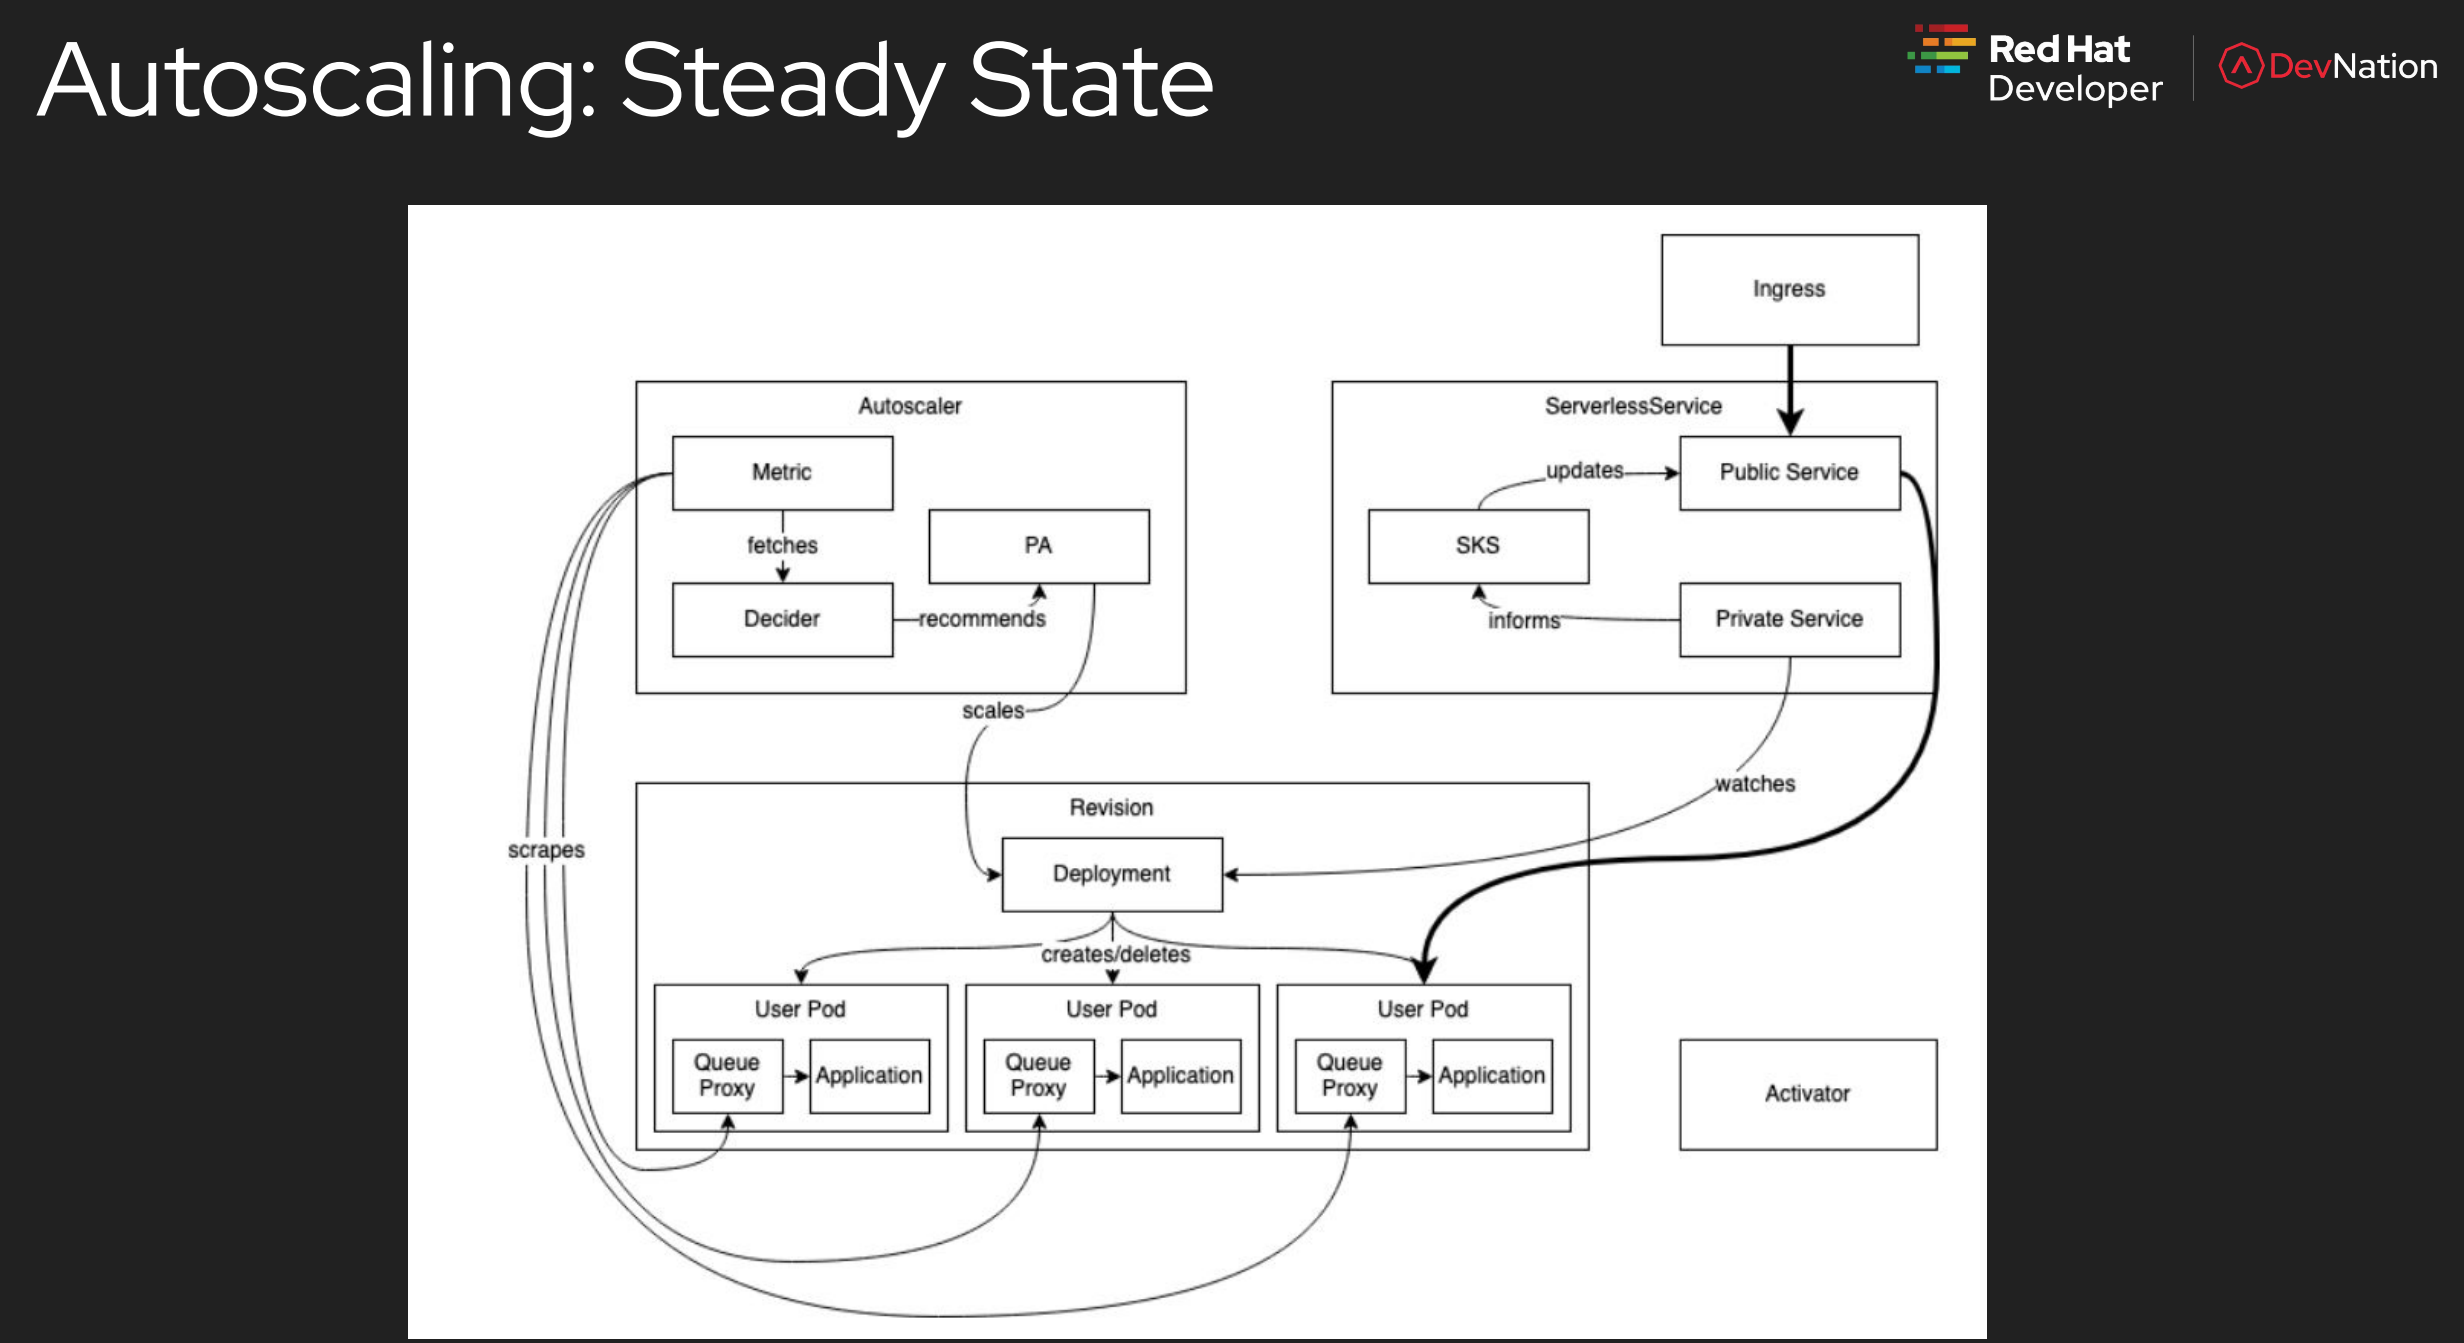
\includegraphics[width=0.5\linewidth]{images/KnativeAutoscaler-2.PNG}
    \caption{Autoscaler : for Normal Traffic }
\end{figure}
\begin{flushright} ref: \textit{\cite{Morie_2020}} \end{flushright}
\end{quote}
\pagebreak
\section{Deployment overhead of Knative}
\begin{flushleft}
Knative is offered over Kubernetes as set of CRDs and Services. Knative framework includes Knative Serving, Eventing. It will also need a Service Mesh. 
These are the required components that must be deployed before deploying any Knative Serverless function.
\begin{itemize}
    \item Service Mesh: It enables secure service-to-service communication and authorization, using sidecars processing secure communication controlled by a central plane. 
The deployment contains set of CRDs, Services, Gateway components etc.
    \item Knative Serving:  Manages deployment, configuration, revision and routing of the Knative application in Kubernetes.
    \item Knative Build: The Knative Build framework is read the Function code and manifest, to prepare a container image, pushing it to the Container Registry.
    \item Knative Eventing: Knative Eventing provides the framework and API to configure and integrate Messaging Channels, Brokers, and Triggers. It facilitates the integration of third-party message brokers like Apache Kafka and Rabbit MQ as event sources.
\end{itemize}
\break
\begin{figure}[h]
    \centering
    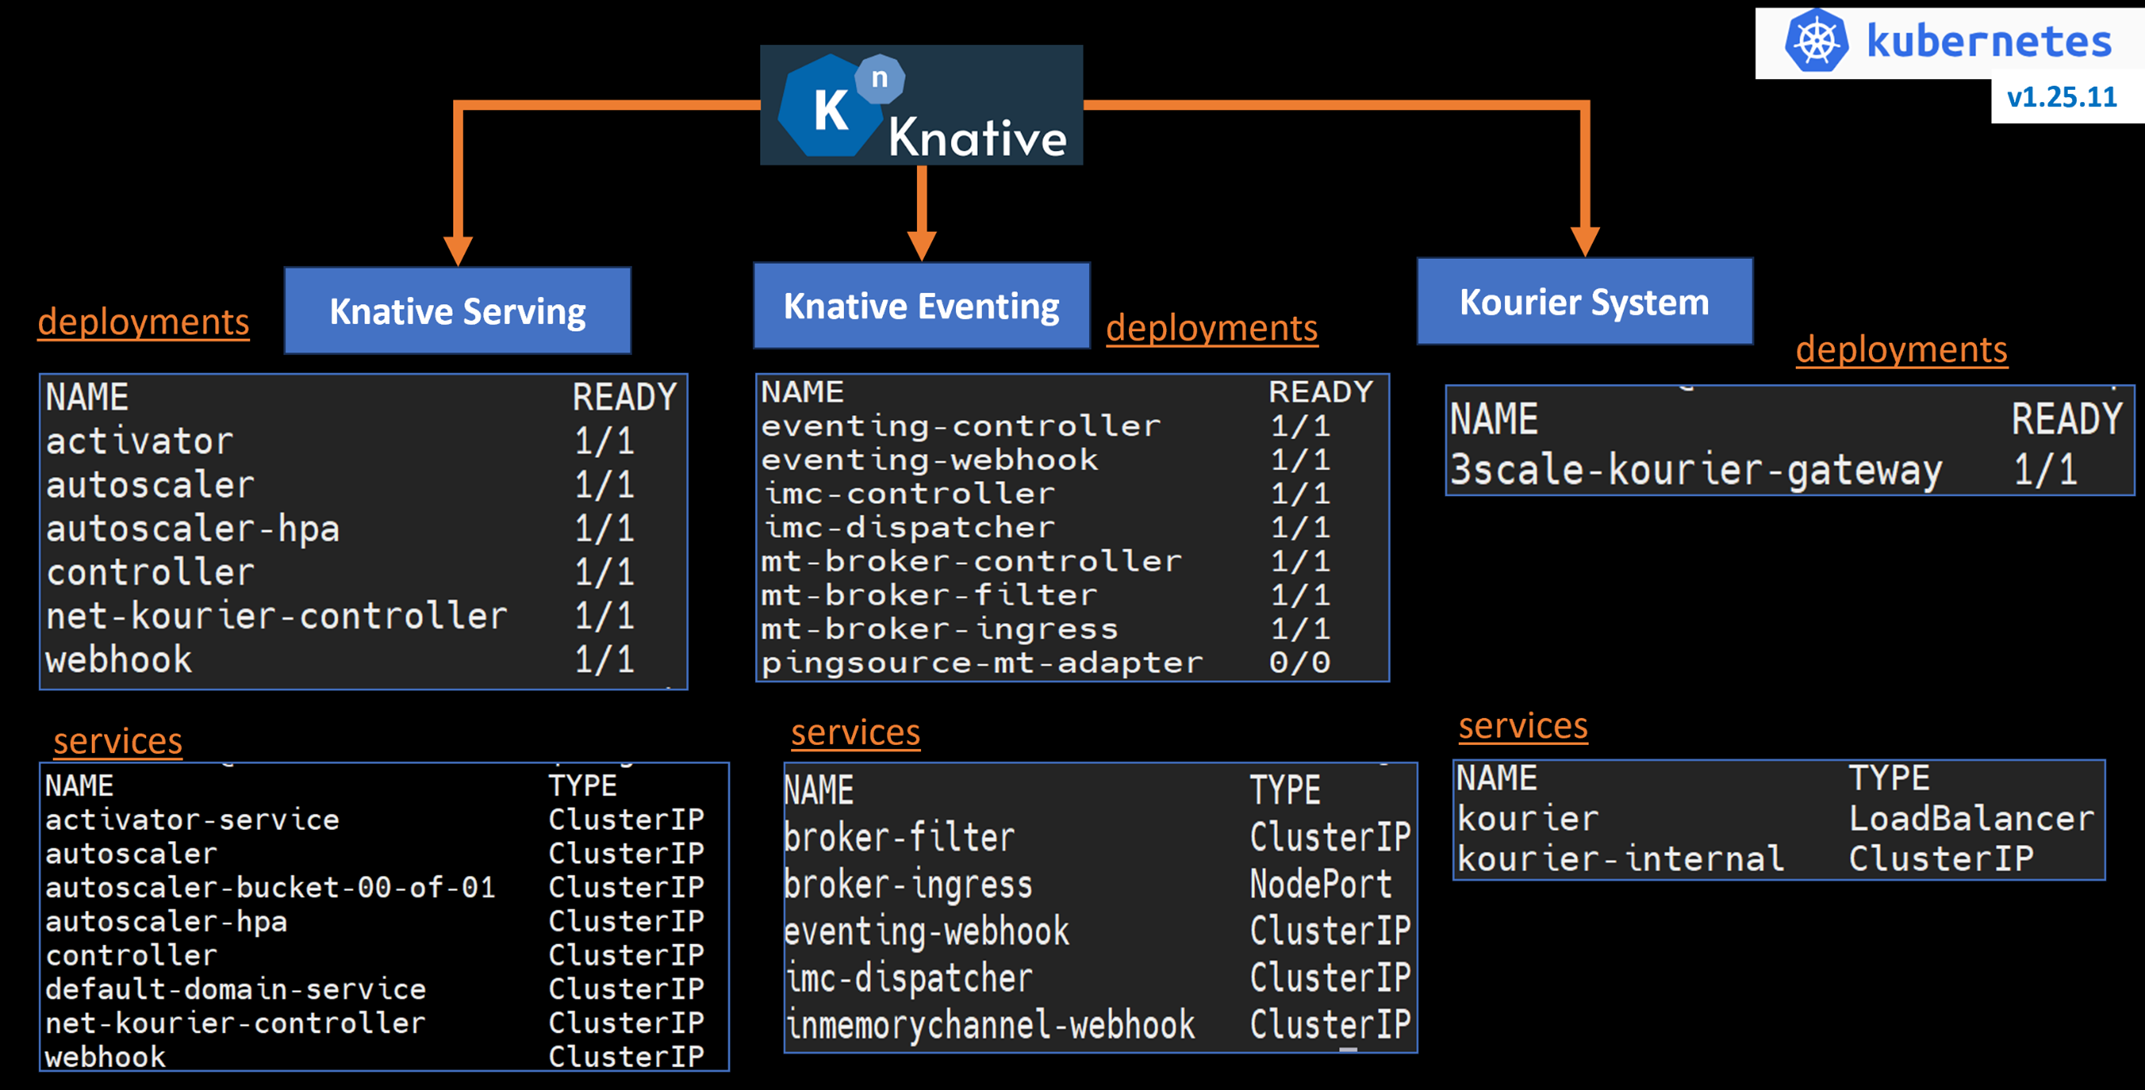
\includegraphics[width=1.00\linewidth]{images/KnativeAllServieces.png}
    \caption{Knative Core Components , PODs and Services}
\end{figure}

\par
The initial deployment of Knative frameworks and components offers complexity and expert understanding of Kubernetes and Knative components. However, these steps can be considered as One of the Admin jobs, automated using CI jobs. The controlled deployment using the YAML configuration file offers greater control and flexibility in preparing the Serverless Infrastructure.

\subsubsection{Higher Infrastructure cost}
Since the Knative framework requires many mandatory components and services to be deployed and running, it increased the physical hardware requirement of the Kubernetes Nodes to a minimum of “Standard D2 V2” (, which is 4 Core CPU and 14 GB Ram). 
\par
There are at-least 14 different core components, that must be deployed as part of Knative Serving and Eventing. The number of components that will be deployed as part of Knative, will further depend of type of \textit{Service Mesh} deployed. 
\end{flushleft}
\pagebreak
\section{Developing and Event Driven Application}
\begin{flushleft}
Azure Eventing framework provide a production grade messaging service like Event-Grid and Event-Hubs, which supports easy integration to Azure Functions. Event Grid enables clients to publish and subscribe to messages over the MQTT, \gls{HTTP} and other protocols. Azure Messaging Service also allows subscription and filtering of events and triggers to registered endpoint or Sink. The Sink can by Azure Serverless Function, Azure Webhook and Services. 
\begin{figure}[h]
    \centering
    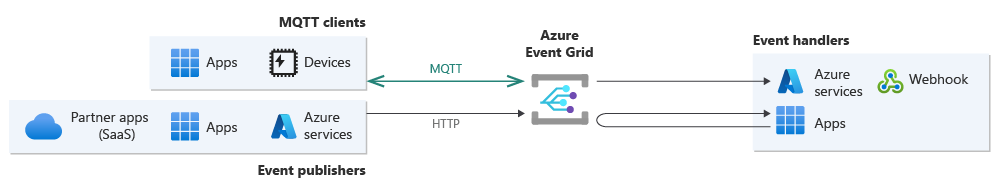
\includegraphics[width=1.00\linewidth]{images/general-event-grid.png}
    \caption{Azure Event Grid}
\end{figure}
 
\par
Knative Eventing, already explained in section 5.3, provide the framework to develop an event driven application. Knative eventing provide integration with other third-party messaging frameworks, like Kafka, NATs, etc. It distinguished itself from Azure function by providing a Broker, providing an abstraction over different event channels. 
\hfill\break
Both Azure and Knative intend to isolate the functional code and configuration from messaging infrastructure. Knative provide event "Brokers", which is an abstraction over different messaging channels. 
\hfill\break
The Event Triggers in both Azure and Knative, subscribe to events, filters and routes it to the SINK. These subscription are externally configured without impacting the functional code. Messaging formats like Cloud-Events is used to keep the function code independent and portable. Filtering is done on Cloud-Event attributes. 
\end{flushleft}
\pagebreak
\section{Workflow Orchestration }
\begin{flushleft}
Both Azure Function and Knative provide options to create a Workflow. These workflows are created using Eventing Framework which includes Event Source, Sink, Event Brokers, and Triggers. 
\hfill\break
The workflow orchestration consumes events from the message broker and triggers events which invokes Serverless function. The Serverless function receives event in CloudEvent format, it can return a transformed event back to the broker or channel for next stage of processing
\hfill \break
There are 2 types of Workflows created in Knative 
\begin{itemize}
    \item Parallel
    \item Sequence
\end{itemize}
\textbf{Parallel Workflow}, offered by Knative is a set of CRD that defines a set of branches. Each branch contains filters and subscriptions. Knative Workflows creates channels and Subscriptions under the hood. Both Filter and Subscription refer to a Knative Service Function.
\hfill \break
\textbf{Sequence Workflow}, offered by Knative is also a set of CRD that defines an order list of functions that must be invoked. Each step creates a filter and transforms events as they are passed. Knative Sequence workflows also create Channels and Subscriptions under the hood.
\end{flushleft}
\pagebreak
\section{Simple Use-Case}
\begin{flushleft}
To demonstrate and test the features of Knative and Azure Function, a simple Use Case is created demonstrating an Event-Driven Microservices and Workflow.
\hfill \break
The use case starts with generation of an invoice by the clients, making a REST call to the Event Grid or Broker. The Application will consume the event and update the status of invoice as \textbf{NEW}.
The updated invoice is published back to the eventing system, triggering the other Microservices to consume and register it to the system, republishing the invoice with status as \textbf{PENDING}. The client can pay for the pending invoice by POSTing a cloud event with invoice data and status as \textbf{PAID}. the Application will now consume the paid invoice and validate it. The result of validation is republished with invoice updated status. If the balance left after payment is zero, the status is updated as \textbf{CLOSED}, if the balance is greater then zero, the status is updated back to \textbf{PENDING}
\begin{figure}[h]
    \centering
    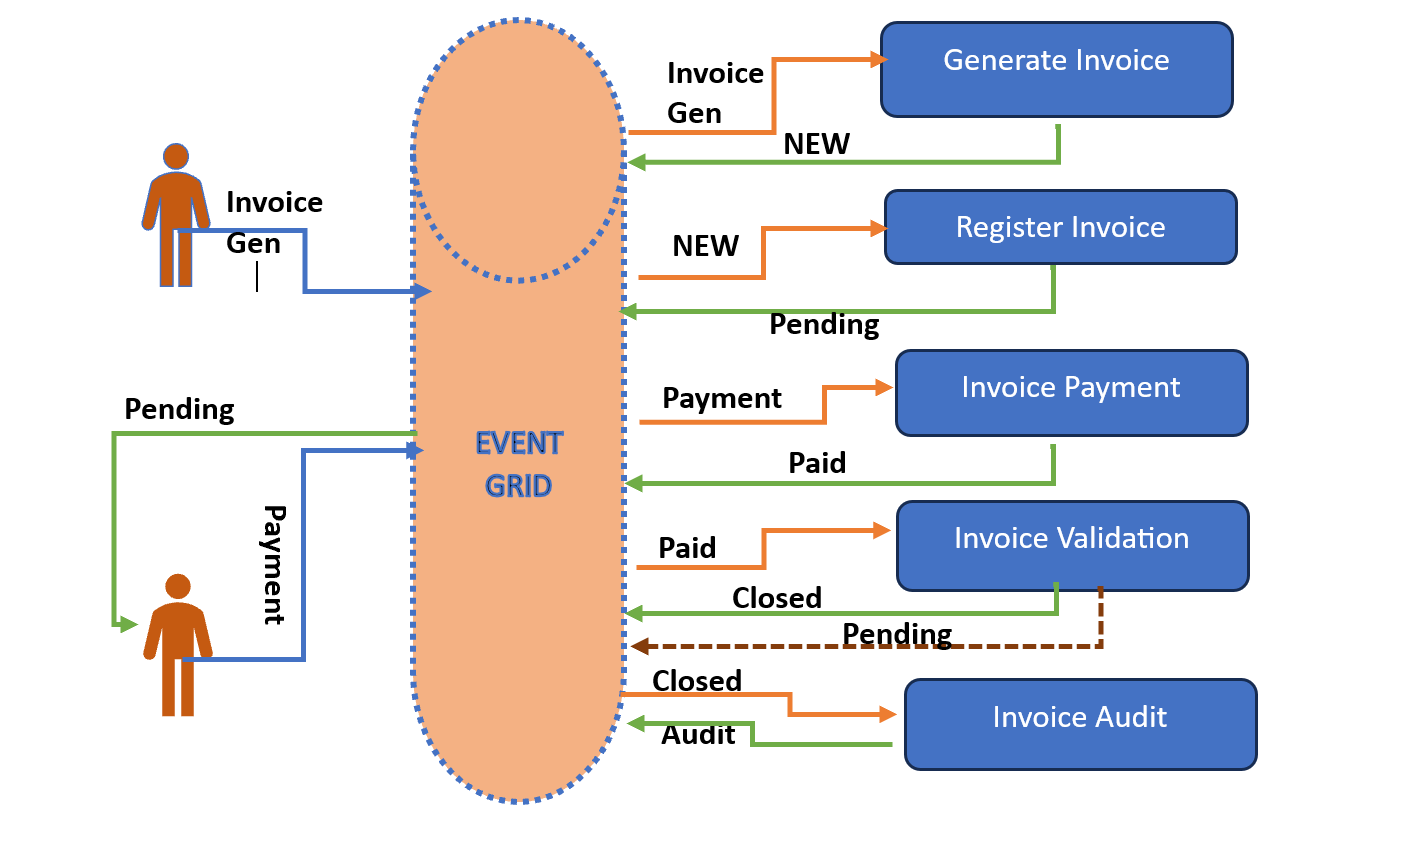
\includegraphics[width=1.00\linewidth]{images/UseCase.PNG}
    \caption{Use Case}
\end{figure}

All these stages will require unique stateless, Serverless, Event Driven Microservices. The Status and Type of Invoice will act as filter, triggering different Microservices to react. 
\break

\subsection{Application Code base}
We have 2 code bases one for Azure another for Knative. Both involves CloudEvent as intermediate data structure. The Logical code is same for Knative and Azure. Deployment process will be different.
\par
\textbf{Azure Function:}\\
\url{https://github.com/AINULX00159358/InvoiceManagerAzure} \\
\textbf{Knative Code base}\\ 
\url{https://github.com/AINULX00159358/InvoiceMgrKnative}\\
\textbf{Test Scheduler code base}\\ \url{https://github.com/AINULX00159358/InvoiceMgrTestScheduler} 

\par
"GitHub Action" automates the deployment of Azure Serverless Function by triggering the \textbf{GitHub Action}, whenever the source code is updated. The Github's \textit{"Action"} executes the Workflow YAML file located in .github \textbackslash workflows folder. The result of execution is a Zip deployment of Azure Functions to the Functional App. The \href{https://github.com/AINULX00159358/InvoiceManagerAzure/blob/main/.github/workflows/main_invoicemgrapp.yml}{workflow file} .

\par
Knative Serverless require docker image, as such Knative Build will create a docker image pushed to a public docker repository (, in this case it is \textit{docker.io}). This is automated using GutHub Workflow YAML file for "InvoiceMgrKnative", which is called by GitHub Action. The \href{https://github.com/AINULX00159358/InvoiceMgrKnative/blob/main/.github/workflows/buildAndPush.yml}{workflow YAML file}. 
\par
Knative deployment is done using a shell script, which calls Azure Function \gls{CLI}. \href{https://github.com/AINULX00159358/InvoiceMgrKnative/blob/main/deployment.sh}{deployment.sh}

\begin{verbatim}
kn_service_create() {
   kn service create $1 
   --env STARTUP=$1 \  
   --image x00159358/invoicemgrimg:latest \  
   --pull-policy=IfNotPresent \
   --label app.solution=invoicemgr \
   --request cpu=500m,memory=512Mi \
   --limit cpu=1000m,memory=1024Mi \
   --scale-metric=rps \
   --scale-target=150 \
   --scale-utilization=95
}
# Function Name is provided as parameter.
# For each function there is a Javascript file will be the env. param STARTUP
# On start NPM will load the Javascript file passed in STARTUP env. variable
\end{verbatim}

The Knative Service will pull the docker image from the registry only once, since 'pull-policy' is set to '\gls{IfNotPresent}'. 

\subsection{Application Design}
The Use Case for Invoice Management System requires an Event Driven Application Design, where each stage managed and processed by stateless, singular function Microservices. 
 \par
Invoice status will be updated in every stage. The cloud-event's attribute "Type" will be mapped to Invoice Status. Cloud-Event's attribute "Type" is used for routing and filtering events to specific Microservices, by the configured Trigger.
\par
Event Grid or Knative broker (with event channel) with its Trigger and filter will act as Orchestration of invoice data to different Microservices. Both Event Grid and Knative broker exposes an web accessible URL, allowing client to POST Cloud-Event data using \gls{HTTP} protocol.
\par
Serverless application, perfectly fits the Microservices requirement. It is stateless, isolated, event driven and only process single function. Their endpoints are exposed and configured in the Event Triggers, with Invoice Status acting as a filter. 
\hfill\break
Serverless offering from either Knative or Azure can be utilized for this design.

\subsubsection{Test Code}
A Test Code is deployed as Simple Kubernetes \gls{POD}, which will start by POSTing client Invoice Request to the Broker Endpoint at different \gls{TPS} like 30, 60, 100 etc.

\subsection{Execution of Test code}
A Test Code is created to request generation of Invoice by making and REST calls to Knative Broker or Azure Event-Grid, using cloudevent schema. The test code is capable of sending Cloudevent at the required rate to simulate regression. 
\par
The Test code is packaged and pushed as Container Image, in \gls{OCI} format, to the Docker repository. The Test application can be deployed as Kubernetes \gls{POD} or Azure Container Application, with required arguments and properties.
\end{flushleft}
\pagebreak

\section{Metrics}
\begin{flushleft}
Both Azure Functions and Knative provide default metrics which is collected and exposed by tools like Prometheus or Application Insight. The application code also provide E2E latency metrics, calculating time taken from generation of invoice to completion of payment. 
\par
Azure Portal provides options to view live metrics of Azure Functional App, as shown in figure ~\ref{azure_live_metrics}

\begin{figure}[h]
    \centering
    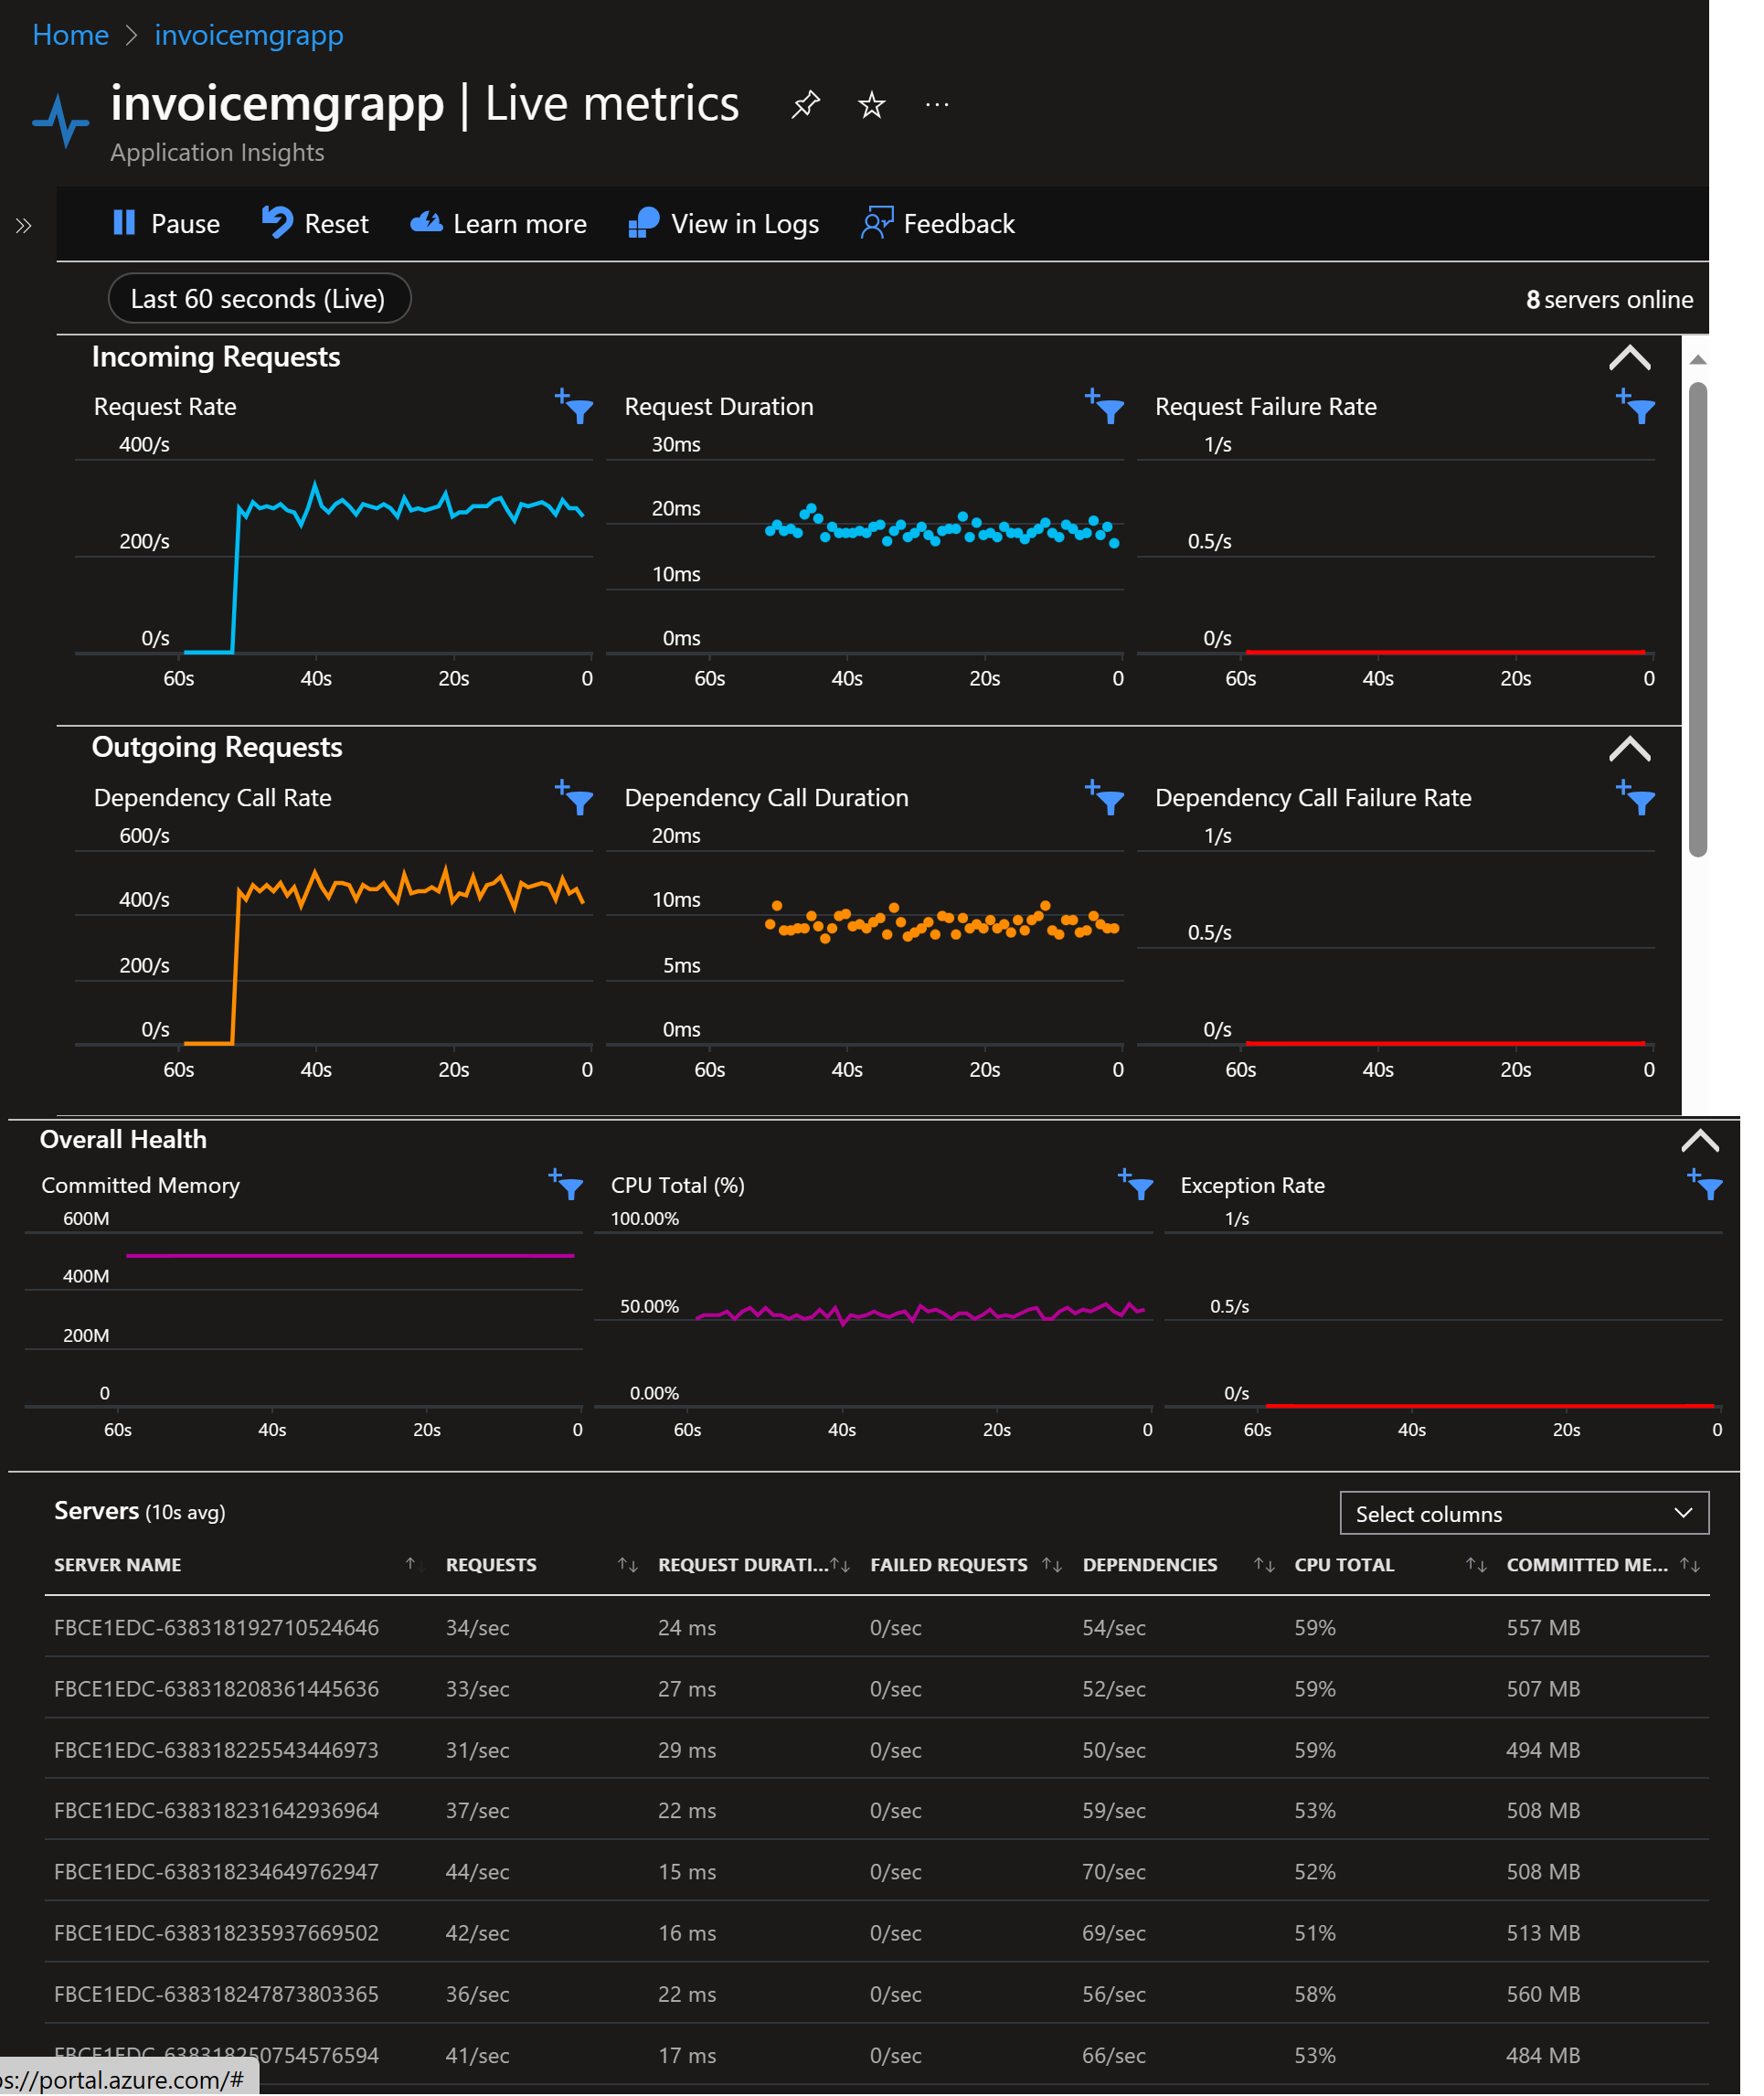
\includegraphics[scale=0.5]{images/AzurePerfCapture/liveMetrics.png}
    \caption{Metrics: Azure Live Metrics}
    \label{azure_live_metrics}
\end{figure}
\pagebreak
\par
Figure ~\ref{azure_live_metrics} , shows Azure Function App is subjected to average 400 \gls{TPS} request. There no failure of request. Request latency for each calls was between 15 to 20 milliseconds.
\hfill \break
The metrics shows average resource usage for all Serverless containers initialized during the Test.
\break

\subsection{Azure Function Cold Start metrics}
Since request for generation of invoice was POST'ed to the Event Grid by the Test Code, a view of Event Grid's Topic latency can give some hint on Cold Start latency. This is presented in Figure \ref{event_grid_latency_metrics}

\begin{figure}[h]
    \centering
    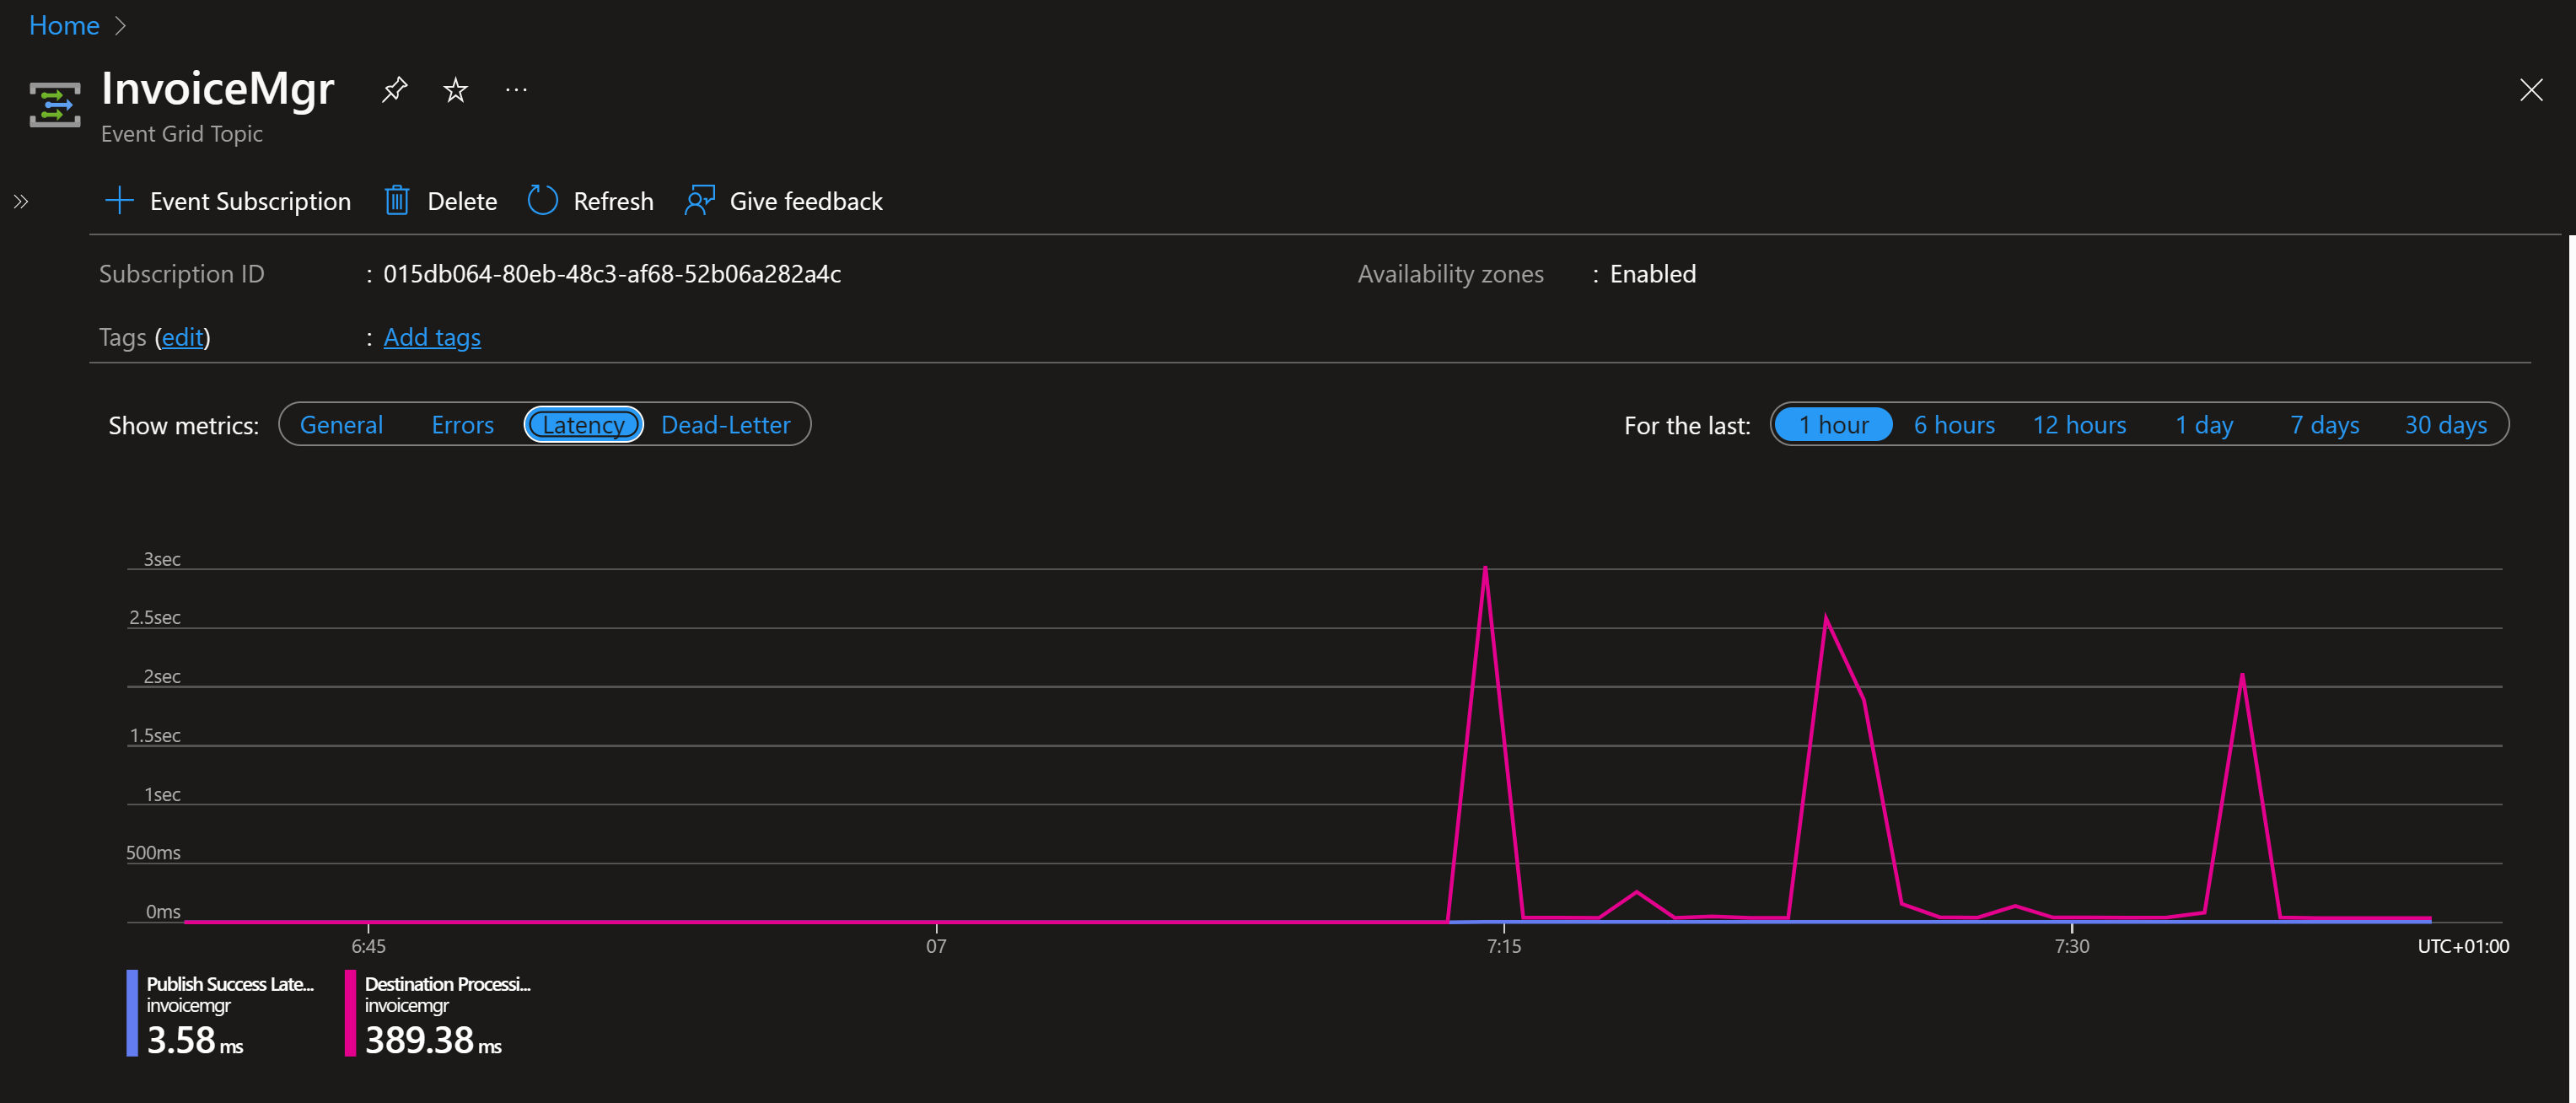
\includegraphics[scale=0.20]{images/AzurePerfCapture/eventgrid-topic-latency.PNG}
    \caption{Metrics:Event Grid Latency Metrics}
    \label{event_grid_latency_metrics}
\end{figure}
\par
The Max latency was between 2 seconds to 3 seconds, which could be attributed to cold start. This is echoed by the Latency experienced in Knative Function "invoicegenerator" , as shown in figure 
\begin{figure}[h]
    \centering
    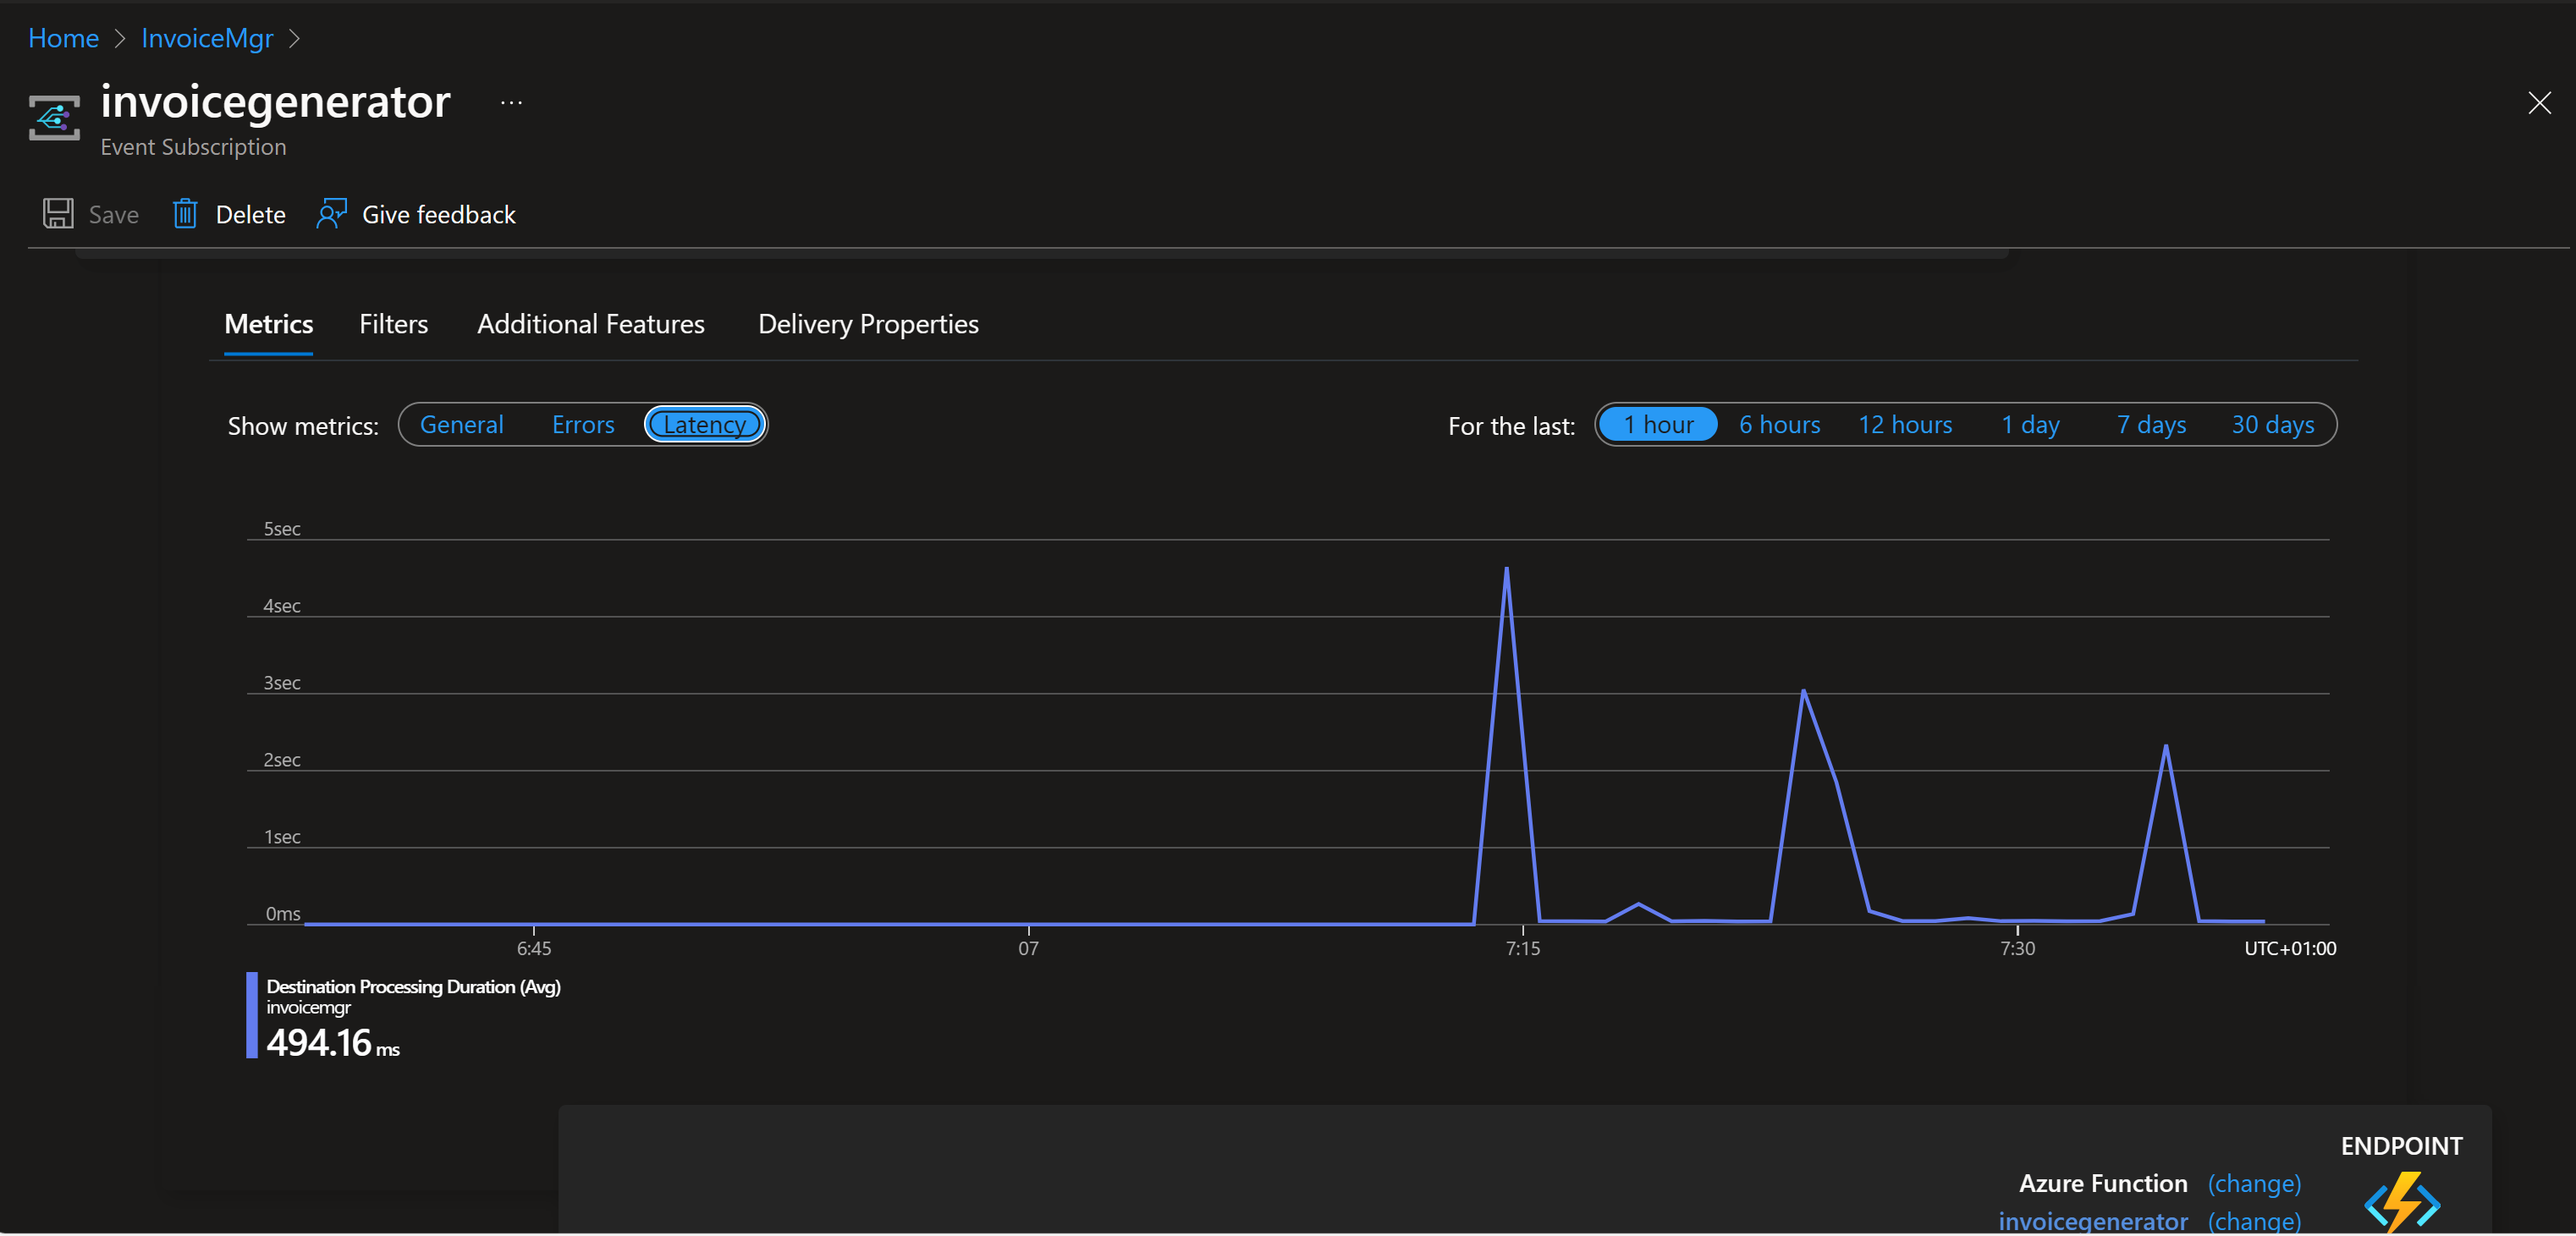
\includegraphics[scale=0.20]{images/AzurePerfCapture/invoicegenerator-event-latency.PNG}
    \caption{Metrics:invoice generator Latency Metrics}
    \label{invoice-generator_latency_metrics}
\end{figure}
\par
\subsection{Metrics Recorded for Knative Application}
These metrics are captured from Prometheus, These startup metrics is evaluated by taking a delta of time in Seconds when \gls{POD} is scheduled and achieved a ready state. This gives the "Cold-start" latency.
\subsection{Knative Metrics: First Initial Deployment}
First initial deployment involves pulling docker images from the repository and start the pod. First deployment will also have time spent in creation of services and service-proxy, registration of public endpoints to registry.

\begin{figure}[h]
    \centering
    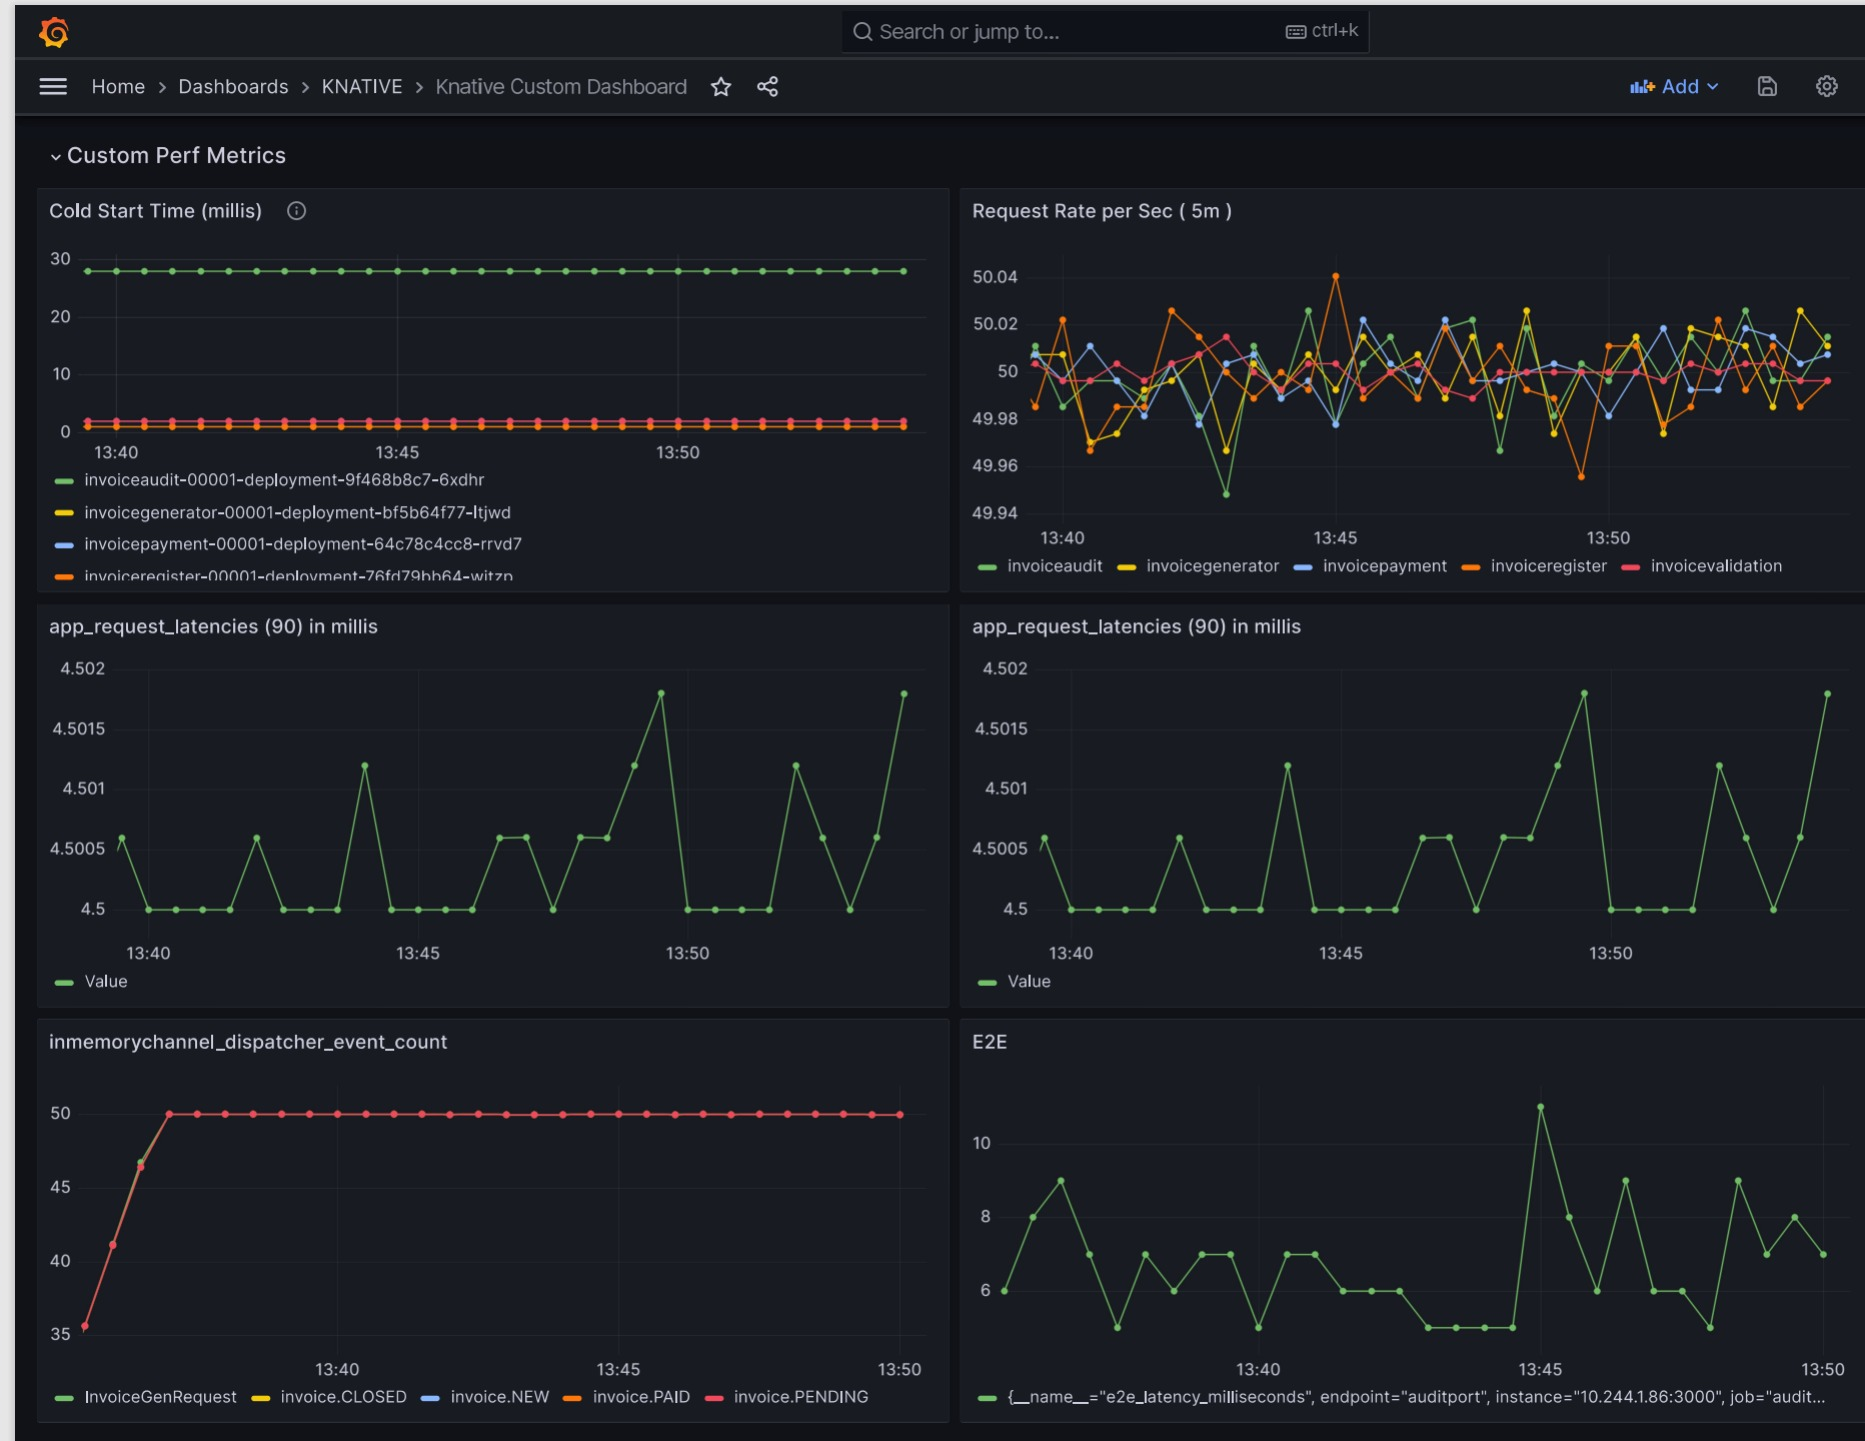
\includegraphics[scale=0.5]{images/Grafana/Grafana_Cold_Start_FirstDeployment.PNG}
    \caption{Metrics: First Initial Deployment}
    \label{grafana_first_initial_deployment}
\end{figure}
\par
Metrics shows higher cold Start time of 30 sec on first initial deployment, because of time spend in pulling image from Repository. Since we are using the same image for all other services, subsequent initialization of services will undergo "Warm Disk Start" with Cold Start time of 1 sec.
\subsection{Knative Metrics: Warm Disk Start}
Once the image is pulled, subsequent deployment will reuse the image. This stage can be considered as "Warm Disk start".
\pagebreak
\begin{figure}[h]
    \centering
    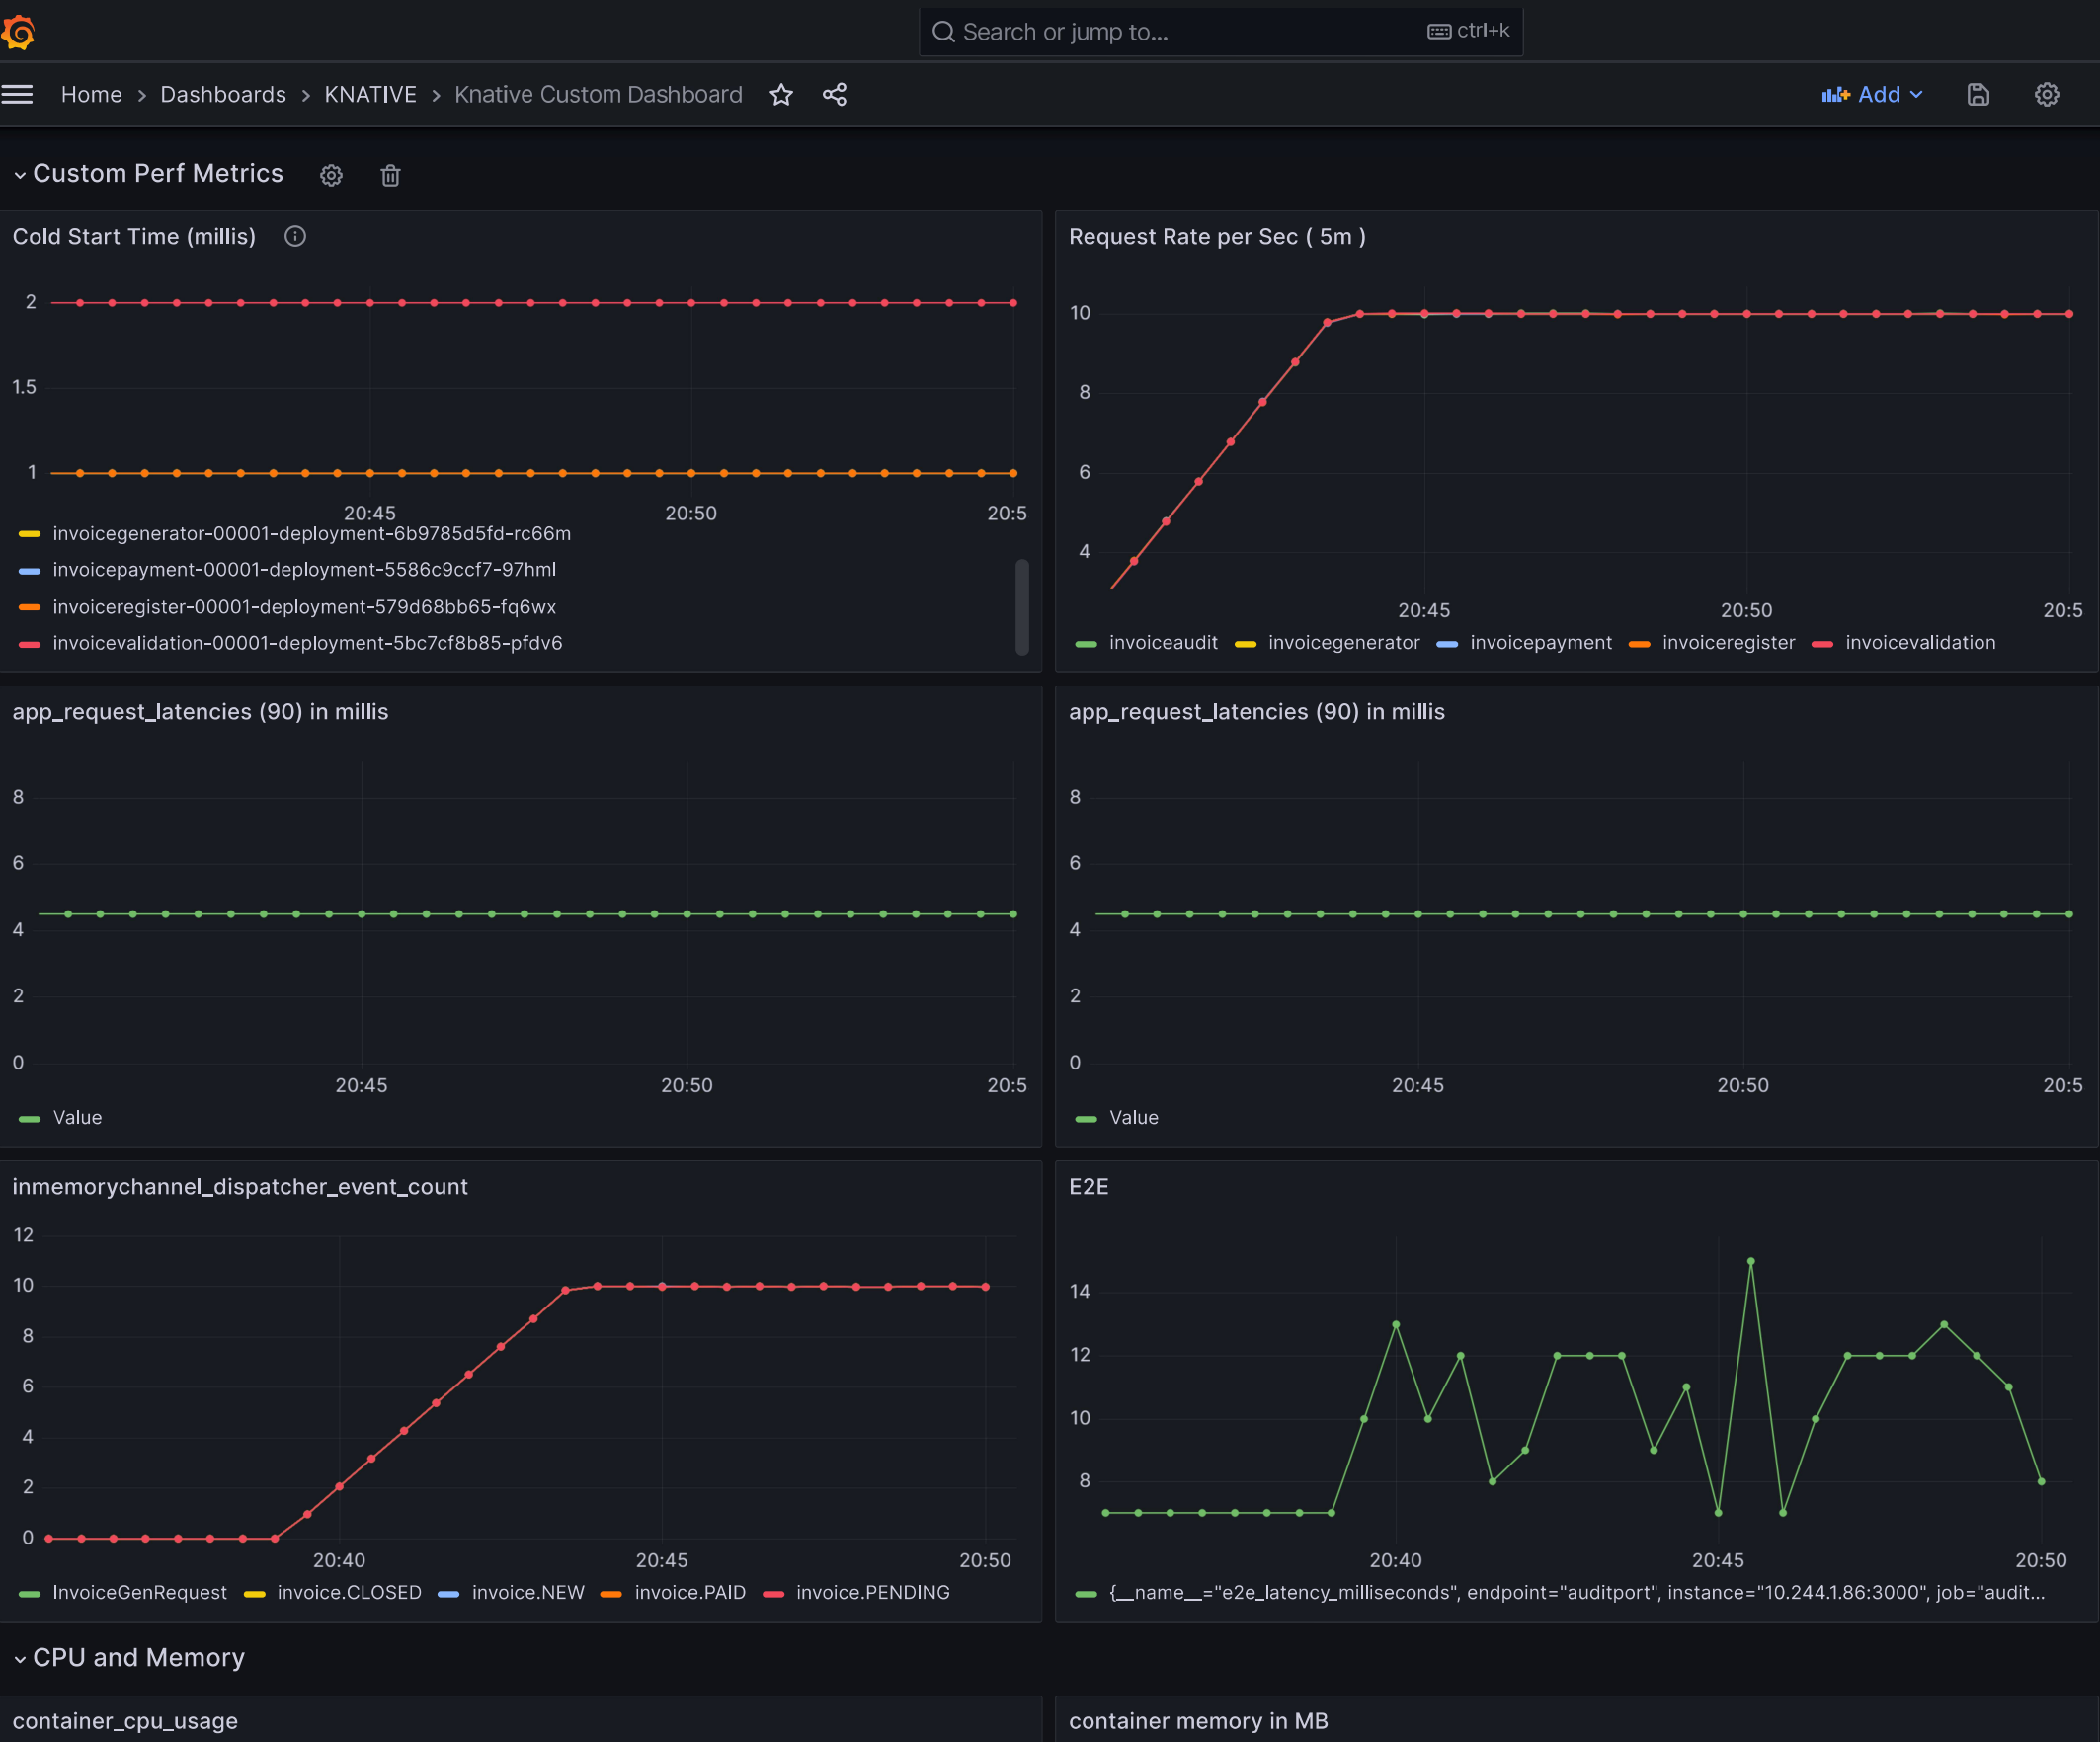
\includegraphics[scale=0.5]{images/Grafana/Grafana_WarmStart.PNG}
    \caption{Warm Disk Start}
    \label{warm_disk_start}
\end{figure}
\par
This metrics is collected after sending first Traffic, causing the Pods to Scale from Zero to One. This is the stage of "Warm Memory Start". Application is faster to start avoiding cost of Address registration etc.
\par
Metrics shows reduced cold Start time to one seconds, compared to Cold Start during first deployment, (ref figure \ref{grafana_first_initial_deployment} ). Other metrics like application and e2e latency tends to remain consistent over time.  
\pagebreak

\par
\subsection{Metrics: Application Auto-scaling}
 This metrics is collected after traffic bust, which triggers auto-scaling. Traffic Bust challenged the capacity and capability of Current Kubernetes nodes, triggering scaling of pods. 

\begin{figure}[h]
    \centering
    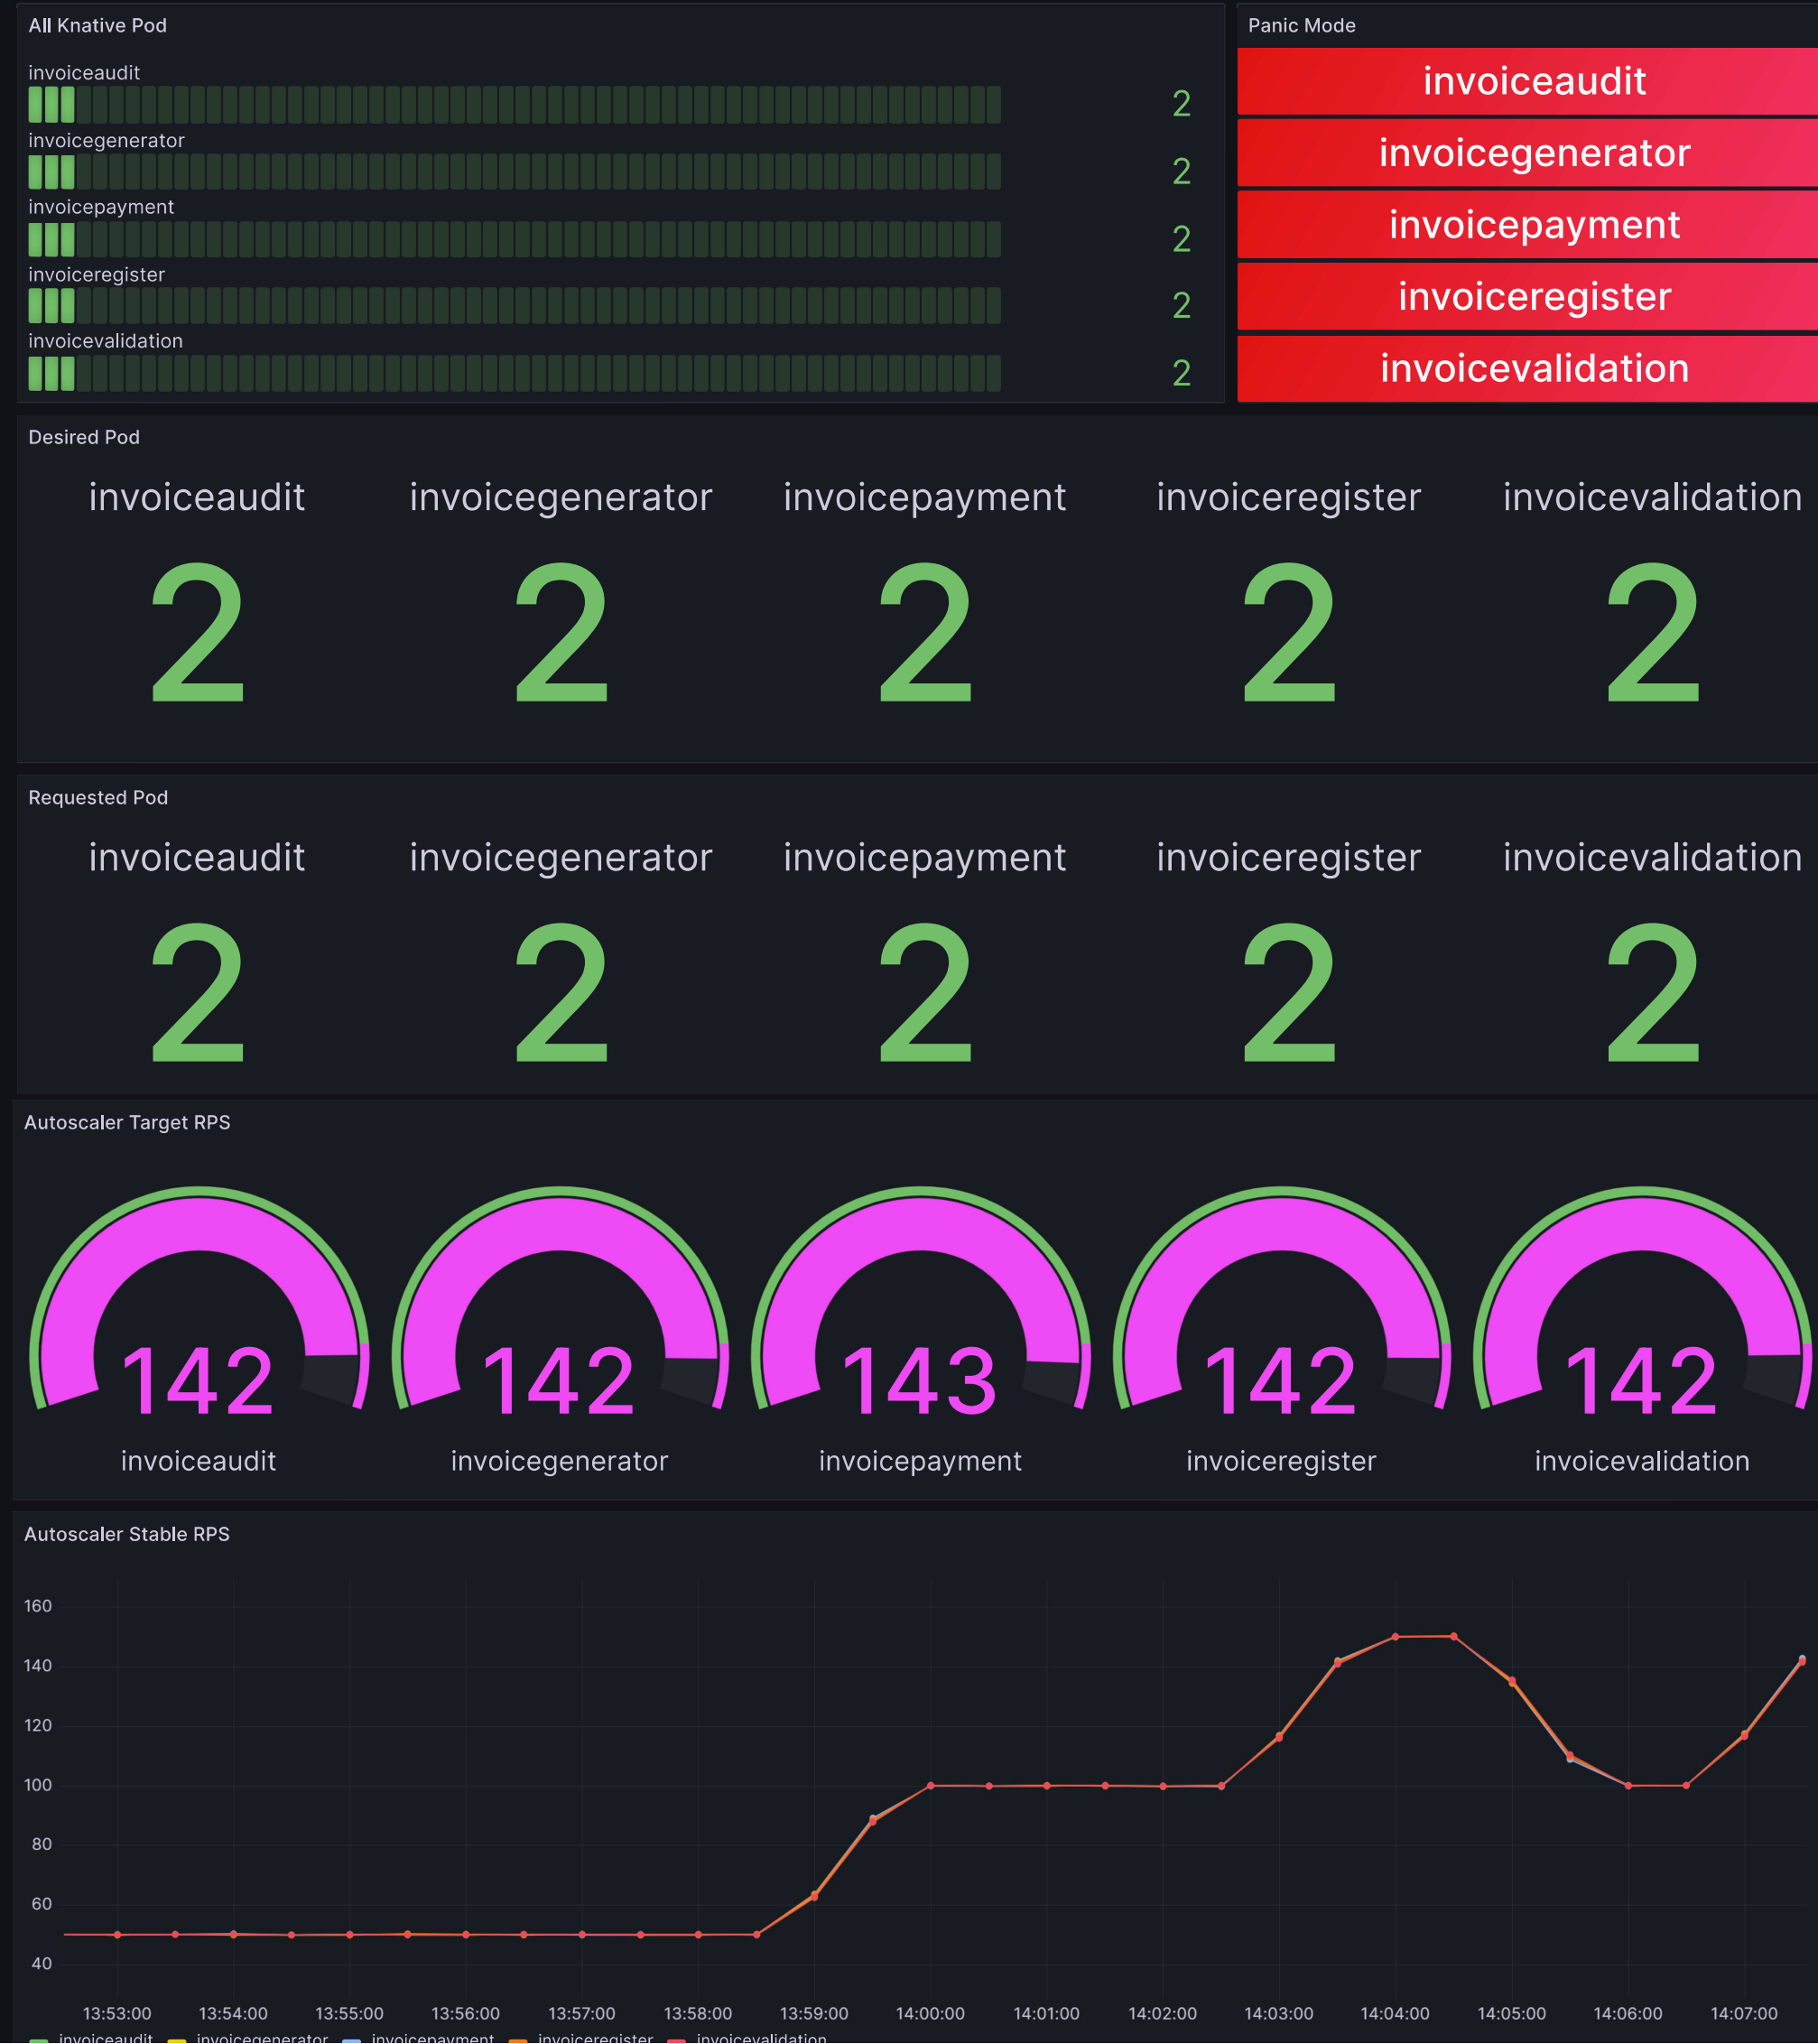
\includegraphics[scale=0.5]{images/Grafana/Grafana_Autoscaling_Panic.PNG}
    \caption{Knative : \gls{POD} Auto scaling in Panic mode}
    \label{fig:Pod_Autoscaling_panic}
\end{figure}
\hfill\break
The default setting for Autoscaler in Knative is "request concurrency", but for test it was modified to "request per second" (\gls{RPS}).  When the \gls{RPS} touched the 70\% of the threshold value (i.e 200), Autoscaler went in a panic state, requesting Knative Serving to spin more \gls{POD}(s).   
\break
\begin{figure}[h]
    \centering
    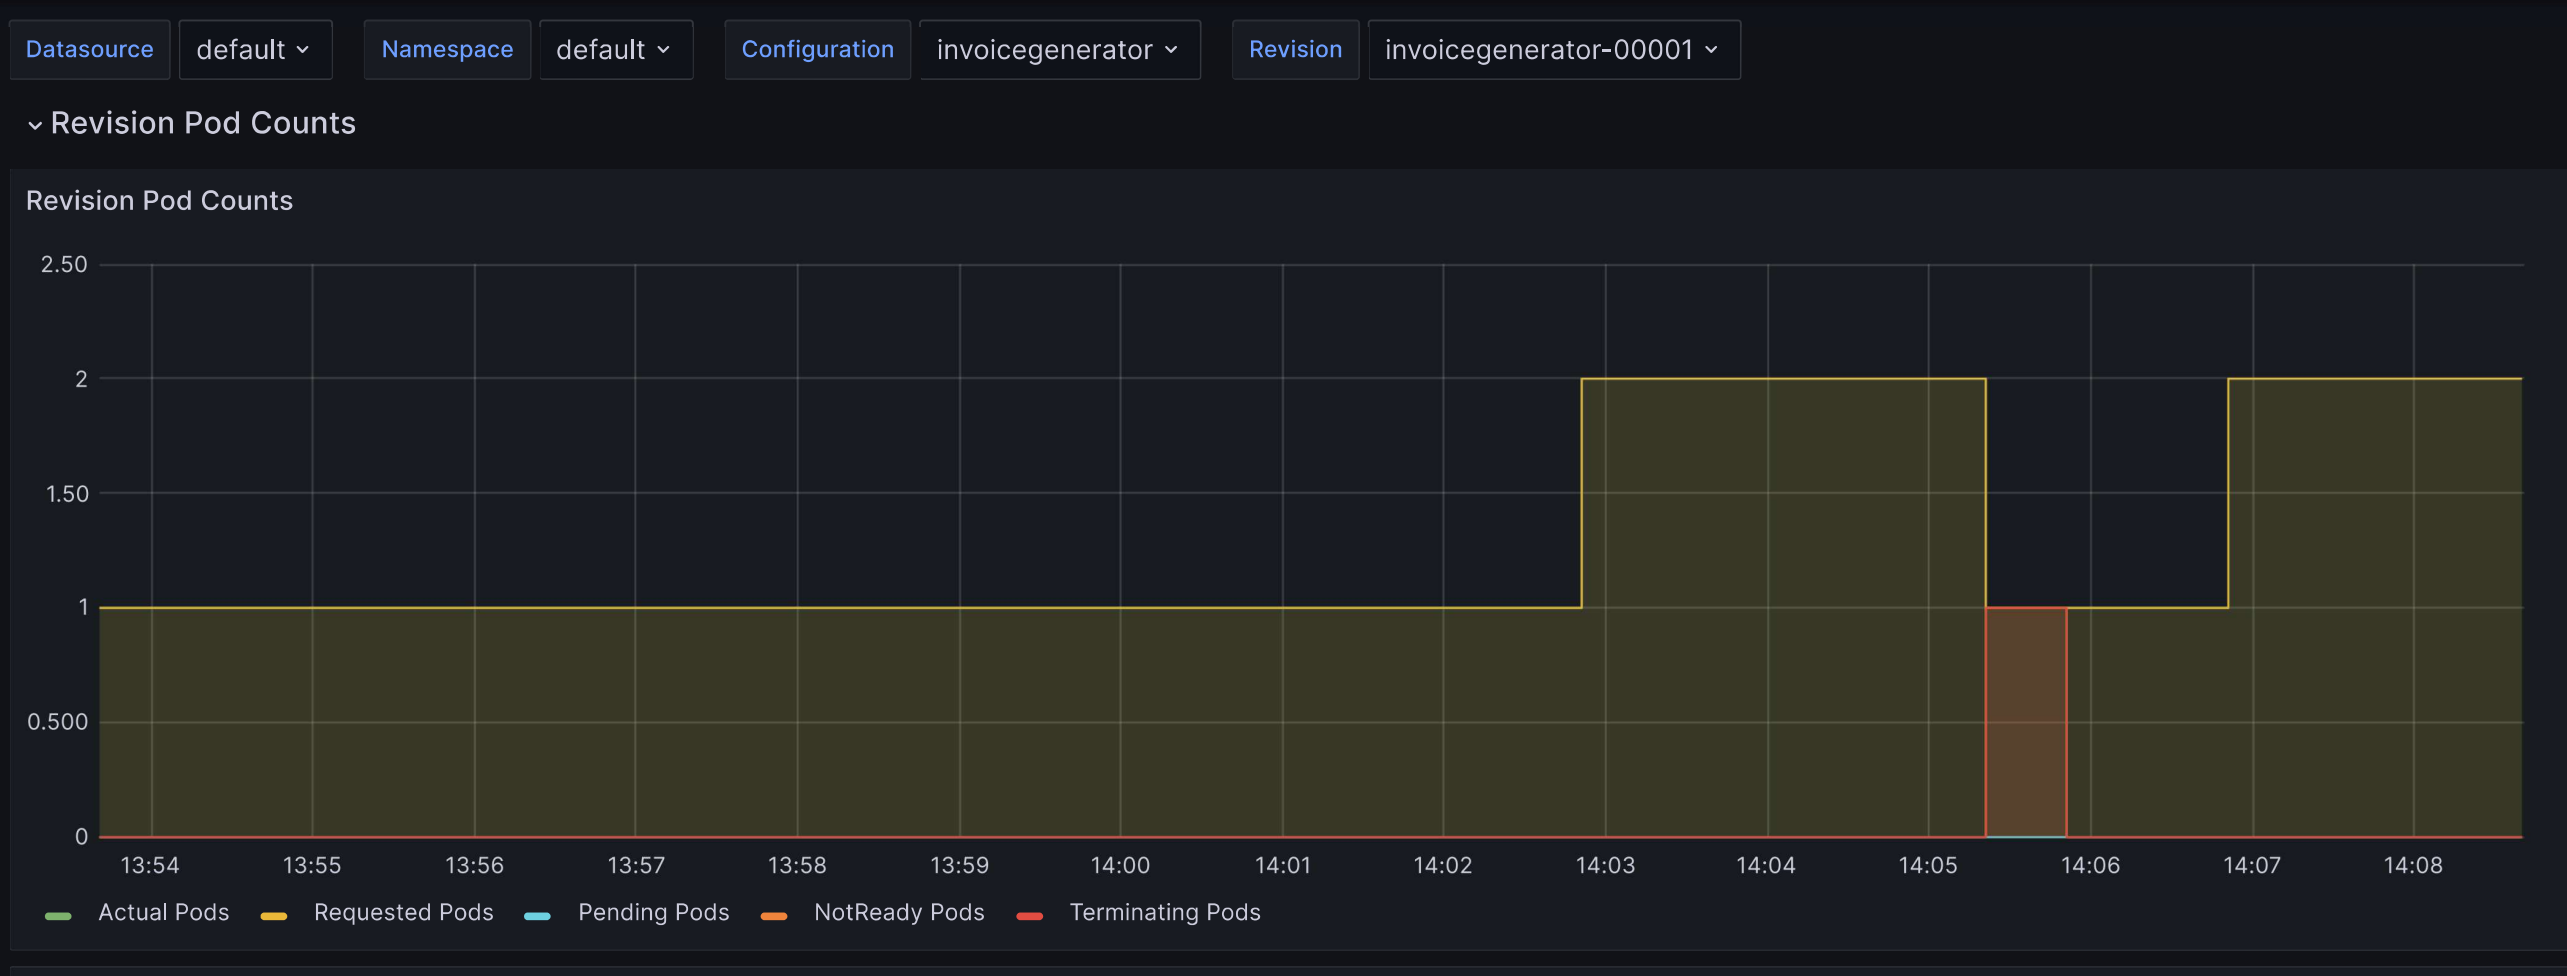
\includegraphics[scale=0.5]{images/Grafana/Grafana_Autoscaling_Knative_Serving_SinglePod}
    \caption{Knative : \gls{POD} Auto scaling in Knative Serving mode}
    \label{fig:Pod_Autoscaling_KnativeServing}
\end{figure}
\hfill\break
Above figure (\ref{fig:Pod_Autoscaling_KnativeServing} ) shows how desired pod for Knative Function (invoicegenerator) increased from one to two, then stabilized back to 1 when traffic normalized. It increased to 2 again when \gls{RPS} increased back to 140+.
    
\end{flushleft}
\pagebreak
\section{Analysis}

\subsection{Deployment}
Knative has an overhead of setting up the Kubernetes cluster, Service Mesh and its required Infrastructure. In production environment a reliable messaging infrastructure like Kafka must be deployed.
\par
Infrastructure cost of setting a proper Knative environment which can support high traffic bandwidth, messaging infrastructure and scalability of Serverless will require provisioning of large capacity nodes.
\par

\subsection{Building as Container Image}

The Knative code must be converted and pushed as docker image to the container registry. 
\hfill\break
Kubernetes \gls{POD} will pull the container image from the registry for initial deployment. Cost of downloading the container image do not effect "Cold Start" as long as Image Pull Policy is set to "\gls{IfNotPresent}". 
\par
In Azure the function build, do not convert the code to a docker image, instead it stores the function files in its file system. The Functional code and runtime is loaded to the Container during execution.
\begin{figure}[h]
   \centering
    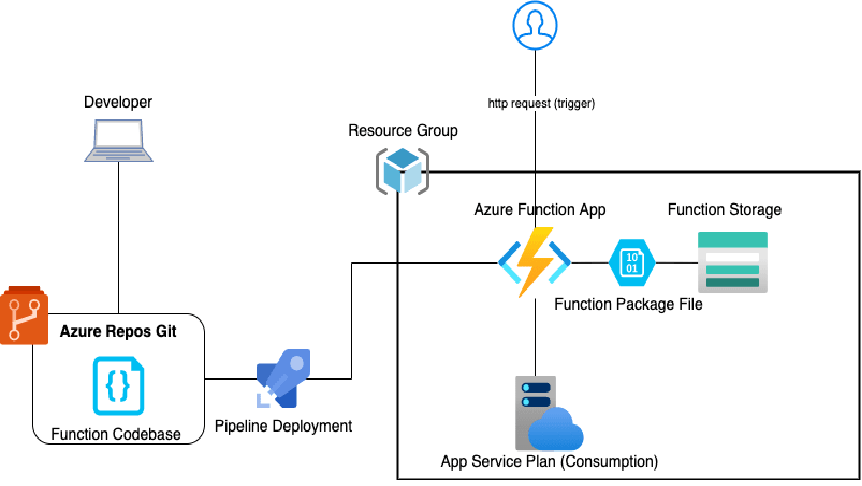
\includegraphics[scale=1.0]{images/AzureDeploymentProcess.PNG}
    \caption{Azure Deployment Process}
    \label{fig:Deployment Process}
\end{figure}



\subsection{Azure's Hosting plan}
Azure's Basic Serverless Hosting Plan is \textbf{"Consumption Plan"}. The Consumption plan scales application on traffic load factor. Customers are charged based on the compute resources utilized. The Compute instances for Functions hosts are dynamically added and removed based on the traffic load factor. Customers are also charged based on function execution.
In production it is recommended to use \textbf{Premium Plan}, which provided larger physical resources, for higher scalability and traffic bandwidth

\subsection{Serverless Costing}
\subsubsection{Knative}
\begin{quote}
    \textit{Knative is best for applications that generate a variable number of trigger events that, over time, stay within established limits. While a single application can meet this requirement, it's more likely met by a combination of three or more applications whose triggers aren't synchronized.}  ( \cite{Nolle_2020} )
\end{quote}
\par
\begin{flushleft}
When there is a large number of Serverless function, any inflation in trigger caused by high or sudden bust of traffic may exponentially increase Serverless cost due to sudden increase in resource utilization and scaling of instances. This against the traditional container applications, which had fixed number of instances, keeping the processing cost constant.
\par
A proper mix of Knative application, can offer better Serverless performance at lower cost than public cloud. But wrong application or poorly sized resource pool can destroy the benefit.
\par
Knative is based on stateless Microservices approach. Business transaction and data is processed by various steps, involving different stateless Microservices. Since stateless Microservices do not preserve state, so do the transaction context. IT teams need to provide their own means to preserve the context which can add to cost of transaction and latency.
\par
The area of responsibility of \gls{SRE} increases when using Knative framework. The \gls{SRE}'s are also responsible for containers, Kubernetes, Service Mesh (like Istio) and Knative Eventing Components (like  Brokers or channels). \gls{SRE}'s are free from these challenges when using Serverless in public cloud.
\par
If the companies already have Kubernetes and "Service Mesh" in their Technology Stack, Knative is just an added extension on it. So for those companies Knative offers a better and affordable solution than their Serverless public cloud provider alternatives.
\par
\subsubsection{Azure Functions}
Azure customer using Serverless Functions, under \textit{Consumption Plan}, is billed based on per-second resource consumption and their executions. Most billing is done using "Pay As You Go Model", where customers pay for compute capacity by second, without any long-term commitments or subscriptions. Customer budget is directly proportional to the increase and decrease in their demand and traffic.
\par
 
Billing for Azure Function Application is subject to the total number of requested processing for all functions in a month. Execution is counted for each time a function is called by the event trigger. There are free exemptions, like 1 million executions per month is free
\par
Customers choose \textit{Premium Plan} for better scalability and no cold-start, with some enhancement in performance. Azure's \textit{Premium plan} for Function App is based on consumption of Core \gls{vCPU} (in seconds) and memory allocation across the running instances.
\hfill\break
Execution charges are exempted under Premium Plan, but it will require at-least one instance to be live and running at all times.
\par
Different pricing tires are available for Premium Plan customers, which provides different combination of \gls{vCPU} and Memory allocated.
\begin{itemize}
    \item \textbf{V2}: 4 \gls{vCPU},  14 GB \gls{RAM} \$0.532/hour
    \item \textbf{V3}: 8 \gls{vCPU},  28 GB \gls{RAM} \$1.064/hour
    \item \textbf{V4}: 16 \gls{vCPU}, 56 GB \gls{RAM} \$2.128/hour
    \item \textbf{V5}: 32 \gls{vCPU},112 GB \gls{RAM} \$4.256/hour
\end{itemize}
\par
\end{flushleft}
\pagebreak
\section*{Conclusion}
\begin{flushleft}
Knative is a Cloud-Native and Open-Source alternative to traditional Serverless offered by public cloud providers like Azure Functions.
\par
Knative becomes a better alternative, for companies who have Kubernetes and Service Mesh in their technology stack, and has an active \gls{SRE} team managing the Kubernetes Cluster. 
\par
Azure Function becomes a choice when companies want to avoid the management overhead of Kubernetes Cluster and Service Mesh. In production, it is recommended to use the "Premium plan" to avoid cold start, which comes with added cost to the infrastructure. 
\par
To summarize, Both Knative and Azure Function are better solutions for Microservices requiring Serverless computing, but Knative offer is diluted by complexity of managing Kubernetes cluster. Azure Function keeps the customers "vendor locked", but are easily managed because Azure takes the responsibility of underlying infrastructure and resources.

\end{flushleft}

\pagebreak

%prints bibliography from bibliography file.
\printbibliography
\clearpage
\printglossary
\end{document}